\chapter{System performance and observations}\label{ch:results}
In Chapter \ref{ch:methodology} both the preparation of the image data actively used within this project and the inner workings of \gls{sys_name} developed using this data were explored. This was crucial as the image data was pre-processed through several stages save for binarization/segmentation of foreground and background, a function pursued by this research. Of this data set, a sub-set of 25 samples was evaluated by experts which informed the performance of multiple features throughout the development process as the outcomes of the system features (e.g. low threshold acquisition, bias application to high threshold selection, etc.) but these evaluations did not effectively serve as measures regarding the ultimate performance of \gls{sys_name} relative to established binarization methods. This chapter will explore how a controlled data set for this evaluation is prepared, the methods to which \gls{sys_name} is to be compared, and the metrics to be used.


\section{Controlled image data used for evaluation}\label{sec:controlled_images}

To evaluate the performance of the \gls{sys_name} it is necessary to evaluate how it behaves under different image conditions, particularly that of image quality degradation. To evaluate the performance of the system under a number of different degradation and image factors it is crucial that these are measurable within the evaluated data set and can be isolated. The isolation of these factors will allow them to be manipulated in a controlled setting to infer the impact each has individually and in combination on the response of the binarization methods (including \gls{sys_name}). Currently, a set of 8 \textcolor{red}{This number will be increased as needed} samples were selected based on the clarity of the perceived foreground structures by visual analysis. The images were then binarized using Hysteresis thresholding using manually selected low and high thresholds to create a controlled starting point where both the intensity and contrast present throughout the images are known and fixed with on the shape and volume of the foreground structures differing between samples. \paragraph{Gaussian blurring} was applied to create another subset using 3D Gaussian blur with the sigma ($\sigma$) being $0.4$ in the in the $z$-axis direction and $0$ in the others. The reason for the 3D Gaussian blurring in the $z$-axis is to attempt to replicate the out-of-focus fluorescence phenomena that are not always completely removed through pre-processing and need to be distinguished as background. A second application of 2D Gaussian blurring is applied with a sigma ($\sigma$) of $2$ to mimic the phenomena that underlie out-of-focus fluorescence and how it can distort structure shape and volume (even weakly). An example of this is shown in Figure \ref{fig:image_blurring_compare}, where dim structures originate from other depths within the 3D microscopy image which is why a centre slice of the image is shown as opposed to a \gls{mip}.

\begin{figure}[h!]
    \centering
    \subcaptionbox{Centre slice of a microscopy image that has been binarized \label{subfig:clean_centre}}{\includegraphics[width=0.49\textwidth]{figs/ch4figs/middle_slice.png}}
    \subcaptionbox{3D Gaussian blurring of the centre slice shown in (\subref{subfig:clean_centre}) \label{subfig:blurry_midslice}}{{\stackinset{r}{}{t}{}{\includegraphics[width=0.1\linewidth, cframe=orange 1pt]{figs/ch4figs/blur_cropping.png}}{\includegraphics[width=0.49\textwidth]{figs/ch4figs/middle_slice_blurred1.png}}}}
    \caption[The effect of the 3D Gaussian blurring on replicating the presence of out-of-focus fluorescence]{The effect of the 3D Gaussian blurring on replicating the presence of out-of-focus fluorescence. A zoomed-in region of interest is shown in the top right corner of (\subref{subfig:blurry_midslice}) with an orange border to show a region where dim structures illustrate out-of-focus fluorescence.\textcolor{red}{I feel that the out-of-focus structures are still difficult to see. Let me know if you think I should try to increase the contrast for this application to improve visibility. Left it as is for now as I spent enough time generating it}}
    \label{fig:image_blurring_compare}
\end{figure}

\subsection{Noise application}
With the images selected and binarized using Hysteresis thresholding, in conjunction with tuned low and high thresholds, a controlled degradation of the image quality is applied to prepare the image for use in performance testing. The two noise profiles that are used are Poisson and Gaussian noise as they are the most commonly occurring noise within microscopy images. When a combination of these noises is applied to the image Poisson is applied first Poisson noise is also referred to as shot noise because it originates from the inconsistent emission and absorption of photons at the microscope photon detector. The received photons are then converted to an electrical signal which could be seen as the raw image signal and Gaussian noise is added to this signal due to electrical and thermal interference from the microscope's electronic components. For this reason, Gaussian noise is applied after Poisson noise in the tests being performed so as to imitate the natural noise phenomena more closely.\paragraph{The Poisson noise} is based on noise values applied to each pixel of the image based on the underlying Poisson distribution. The Scikit-Image~\cite{scikit-image} implementation of the Poisson noise application was first investigated \textcolor{red}{(~\cite{scikit-image} Do you think it is worthwhile to include the name of the exact function?)}. Still, this implementation didn't allow any tuning of the noise intensity through some external parameter thus modifications were made. In the original implementation of Poisson noise, The number of unique intensity values is determined and used to scale the image intensities to fall within a Poisson distribution mean and it is subsequently divided by this unique intensity count to rescale it. After this, the image intensities are clipped to the bounds of the original image's maximum intensity but it was found that without this clipping the intensity values can exceed the original maximum which is believed to be not ideal but an effective approximation. The new variant of this attempts to approximate this implementation of Poisson noise application by replicating the use of the count of unique image intensity values but instead of dividing the Poisson values by the unique intensity count the maximum of the Poisson applied image is used instead to normalize it. After this normalization, the normalized Poisson applied image is raised to the power $p$ where the exponent $p$ is a parameter provided to the function allowing the magnitude of the Poisson application to the image to be scaled. While not perfect this is believed to be a sufficient method to apply Poisson-specific noise which can be tuned in the severity of its effect on the image quality. \paragraph{The Gaussian noise} that was applied used a function provided by Scikit-Image which allows the mean and the variance of the Gaussian noise to be tuned using two separate parameters. For this application, the mean of the noise is kept at the default $0$ but the variance is tuned within a range to affect the severity of the additive noise. A showcase of the Poisson and Gaussian noise profiles being used can be seen in Figure \ref{fig:noise_application_compare} where the original control image is presented as well as the application of Poisson noise, the addition of Gaussian noise, and the combination of both to the microscope image. This is a singular variation of the magnitude of the noise used for each noise profile (Poisson and Gaussian) but serves to illustrate the difference in their resulting effects on the image when used. 
\begin{figure}[h!]
    \centering
    \subcaptionbox{Original binarized image \label{subfig:original_sub}}{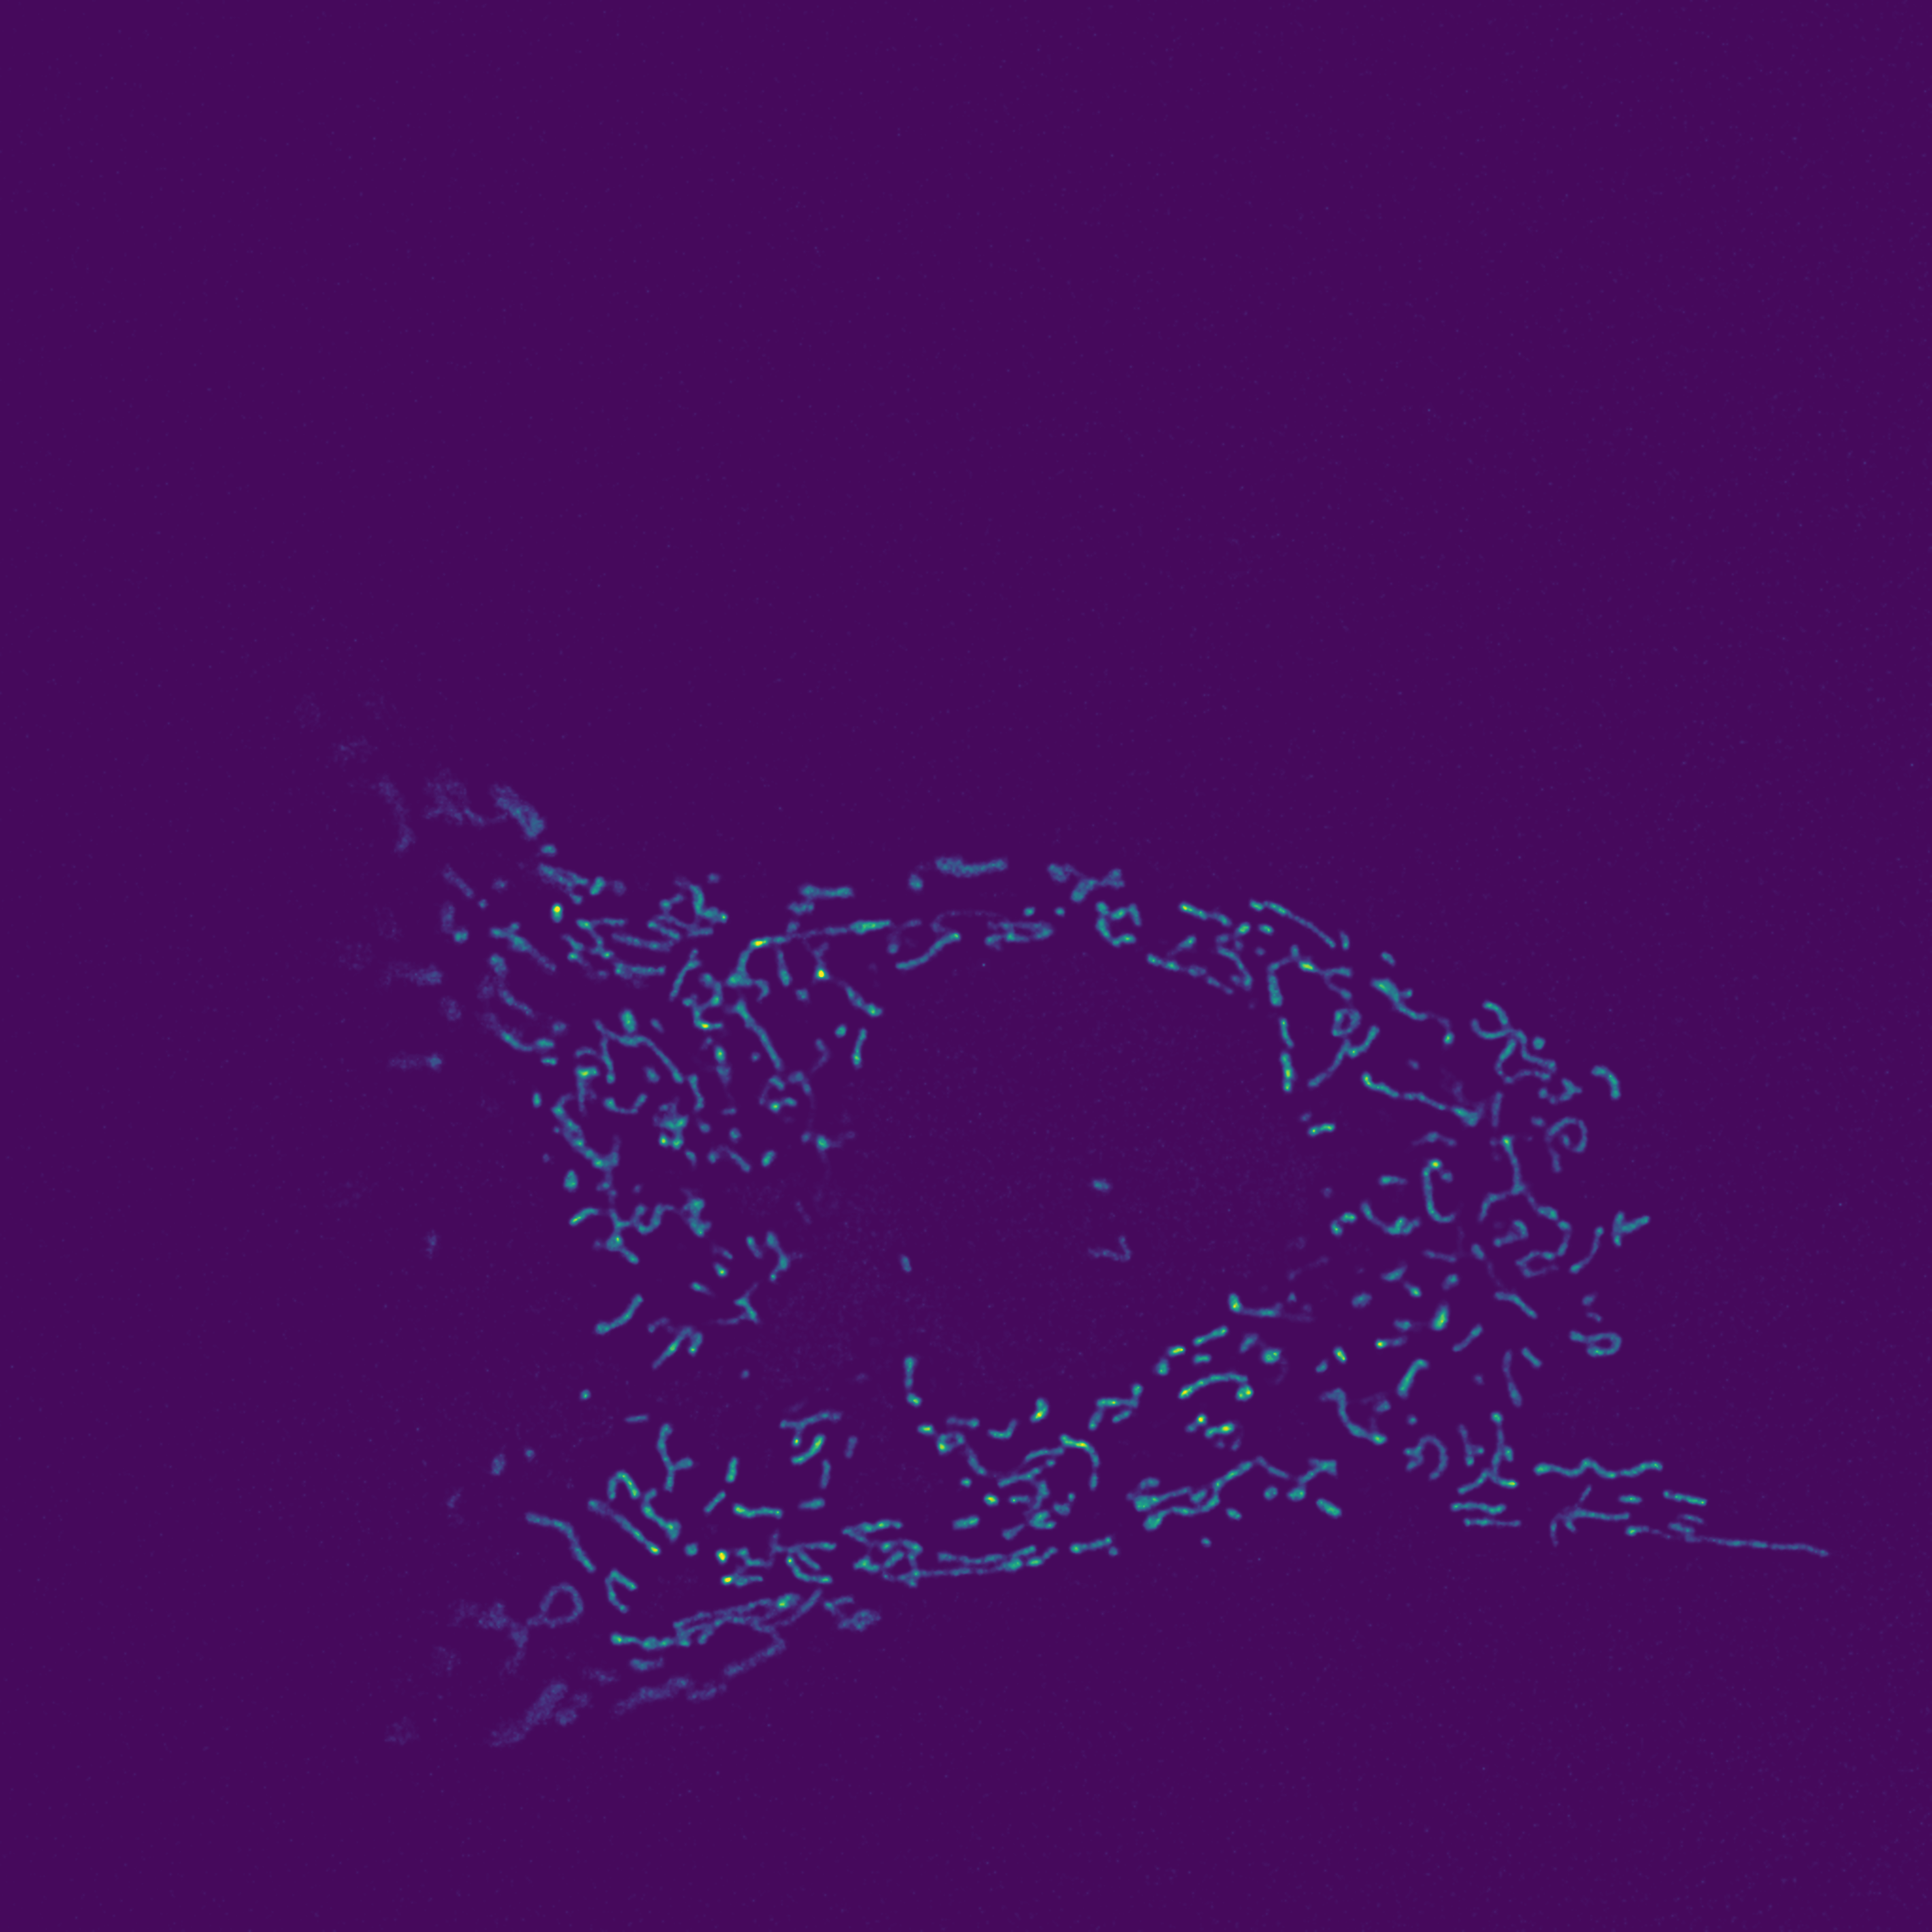
\includegraphics[width=0.49\textwidth]{figs/ch4figs/CCCP_1C=1T=0.png}}
    \subcaptionbox{Applied Poisson noise \label{subfig:poisson_sub}}{{\stackinset{r}{}{t}{}{\includegraphics[width=0.1\linewidth, cframe=orange 1pt]{figs/ch4figs/poiss_window.png}}{\includegraphics[width=0.49\textwidth]{figs/ch4figs/CCCP_1C=1T=0P7G0.png}}}}
    \subcaptionbox{Added Gaussian noise \label{subfig:gauss_sub}}{{\stackinset{r}{}{t}{}{\includegraphics[width=0.1\linewidth, cframe=orange 1pt]{figs/ch4figs/gauss_window.png}}{\includegraphics[width=0.49\textwidth]{figs/ch4figs/CCCP_1C=1T=0P0G0.01.png}}}}
    \subcaptionbox{Combination of both Poisson and Gaussian noise \label{subfig:pg_sub}}{{\stackinset{r}{}{t}{}{\includegraphics[width=0.1\linewidth, cframe=orange 1pt]{figs/ch4figs/poiss_gauss_window.png}}{\includegraphics[width=0.49\textwidth]{figs/ch4figs/CCCP_1C=1T=0P7G0.01.png}}}}
    \caption[Comparison of the different noise profiles applied to the binarized control images]{An image comparison of the effects of the Poisson and Gaussian noise applications to the microscopy images. In this comparison (\subref{subfig:original_sub}) is the original binarized control image which is a single central slice of the 3D microscopy image; (\subref{subfig:poisson_sub}) is the control with Poisson noise applied to it; (\subref{subfig:gauss_sub}) is the control with Gaussian noise added to it; and (\subref{subfig:pg_sub}) is the control with Poisson noise applied and Gaussian noise added.}
    \label{fig:noise_application_compare}
\end{figure}
\paragraph{Image quality measurements} post noise application for each of the control samples using \gls{snr} and \gls{ssim} to explore the degree of divergence from the original control image for each noise variation. The mean of the \gls{snr} and \gls{ssim} values across the range of control images is used to consolidate their results to aid in illustrating the impact the difference in the noise variations has but it is recognised that this is a reductive consolidation as the shape and volume of the objects described by each image vary greatly. This leads to the images not necessarily being comparable as to say that a certain combination of the Poisson and Gaussian noise will impact the overall image quality differently between two images despite the conditions of the noise being applied being identical. This has to be done though for the sake of illustrating the impact that Poisson and Gaussian noise each have on the image quality and to compensate a standard deviation distribution is present to describe the distance between the control samples for each noise combination which can be used to infer how reliable said mean value is. Regardless, what is noticeable is that the \gls{snr} decreases significantly with the increase in Poisson noise intensity while the \gls{ssim} decreases significantly with the increase in Gaussian noise intensity which could be telling of the method by which each evaluates the noisy images. \paragraph{\gls{snr}} is the measure of the signal-to-noise ratio in the noisy image relative to the original binary image on a pixel-by-pixel level thus numerically it can serve as a straightforward but relatively naive measure that cannot consider structural information within the image. For this reason, the Poisson noise applied has a stronger impact on non-background regions (non-zero) and thus leads to relatively greater pixel-to-pixel differences between the binarized control image and the noisy image. Conversely, the opposite appears to be the case for the Gaussian noise where the distortions are present across larger regions of the image but are not as intense as the applied Poisson noise for each individual pixel. \paragraph{\gls{ssim}} evaluates the structural similarity of the image in a manner similar to how a human perceives image quality~\cite{snrVSssim} which considers the loss of correlation, distortion of luminance (or brightness), and the distortion of contrast. Despite the Poisson noise being more intense within the bound foreground regions of the control image there is still considerable contrast present between the noisy structures and the zero-value background, maintaining the noise within the bounds of the foreground structures improves correlation with the control image, and luminance is noticeably diminished only at higher Poisson intensities. Contrary to this robust behaviour against Poisson noise, there is a diminishing response in the \gls{ssim} value observed when the Gaussian noise intensity increases. The Gaussian noise adds a noise layer across the entire image independent of the underlying signal and due to this begins to obscure, even weakly, the foreground structures in the image. It is conjectured that this is likely due to \gls{ssim} evaluating the quality of a noisy image based on how effectively it preserves structural information prior to the noise application but this is not merely the presence of the structures but also the effective differentiation of them from non-structure regions or other structures. It is conjectured that \gls{ssim}'s sensitivity to Gaussian noise is due to how it influences the shape and form of the structures present while Poisson keeps the distortions induced within the boundaries of the foreground structures. \paragraph{The standard deviations} measured in the surface graphs (Figure \ref{subfig:std_surf_c} \& \ref{subfig:std_surf_d}) illustrate the variance in the \gls{snr} and \gls{ssim} between all samples for a noise variation (some combination of Poisson and Gaussian noise) to be evaluated in concert with the results and compensates from the reductive context lost when aggregating the results of the samples using the mean. It is observed that across all measures of the \gls{snr} for any application of Poisson noise, there is a high spread in the \gls{snr} results between the samples further cementing that lack of robustness that the \gls{snr} has. The spread in \gls{ssim} values is interestingly enough not terribly large with it peaking when either one of the two noise types (Poisson or Gaussian) is small while the other is large. It is speculated that this is due to the evaluation of the structures in the image and when the noise is sufficient enough the loss of structural similarity is relatively the same and the performance of \gls{ssim} as a measure is better. From this, it is believed that \gls{ssim} is a superior and more robust measure providing a more reliable evaluation of the quality loss in an image~\cite{snrVSssim} although \gls{snr} will still be used in further performance evaluations despite the shortcomings of it.
\begin{figure}[h!]
    \centering
    \subcaptionbox{The mean SNR distribution across the noise variations}{\includegraphics[width=0.49\textwidth]{figs/ch4figs/Mean_SNR.png}}
    \subcaptionbox{The mean SSIM distribution across the noise variations}{\includegraphics[width=0.49\textwidth]{figs/ch4figs/Mean_SSIM.png}}
    \subcaptionbox{The standard deviation in the SNR values across the samples for each noise variation\label{subfig:std_surf_c}}{\includegraphics[width=0.49\textwidth]{figs/ch4figs/Var_SNR.png}}
    \subcaptionbox{The standard deviation in the SSIM values across the samples for each noise variation\label{subfig:std_surf_d}}{\includegraphics[width=0.49\textwidth]{figs/ch4figs/Var_SSIM.png}}
    \caption[3D surface graphs describing the distribution of the SNR and SSIM (and standard deviation of each) across a range of noise applications]{3D surface graphs describing the distribution of the SNR and SSIM (and standard deviation of each) across a range of noise applications \textcolor{red}{I feel I need to increase the font size in these graphs}}
    \label{fig:noise_application_comparison}
\end{figure}

\section{Performance Evaluation}
The evaluation of the \gls{sys_name} will be performed through a comparison of the outcomes against a number of established methods. Both global and local threshold methods will be compared with Otsu~\cite{Otsu1979ATS} and Li thresholding (``Minimum Cross Entropy'')~\cite{Li_thresh} being the global methods, and Sauvola~\cite{adapt_sauvola} and a local variation of Otsu (Local Otsu) to be used for the local thresholding.\par As discussed in Section \ref{sec:system_biases}, the \gls{sys_name} binarization outcomes can vary depending on the combination of weighting factors used pertaining to the \gls{ihh} distribution weighting bias and the shrinking windowed distribution bias weightings. For this reason, all six permutations of these weighting approaches will be explored with observations regarding their behaviour analyzed.

\subsection{Metric-based evaluation}\label{sec:metrics_compare}
This metric-based approach utilizes the controlled sample images discussed in Section \ref{sec:controlled_images} where the applied noise is known and controlled. Five metrics will be explored which are accuracy, precision, recall, \gls{snr}, and \gls{ssim} where the averages across the samples will be measured as will the degree of deviation based on the standard deviation of the metric results across the samples. The application of the local thresholds in this evaluation employed a window parameter size of 15 pixels as this was the provided default value. It is recognized that the quality of the performance of these methods is dependent on this parameter but it is believed that this may better emulate the naive application of these local thresholding methods by less experienced individuals, particularly in high-throughput applications where the tuning of the window parameter for each sample is non-feasible.

\subsubsection{Accuracy}
For this implementation accuracy is the measure of the number of voxels that are true positive or negative outcomes compared to the original image prior to noise adjustments. This is a measure of the count of correctly labelled voxels (foreground or background) compared to the sum of all voxels across the image where a value closer to 1 describes the proportion of the image that is correctly binarized.

\paragraph{Established methods} Shown in Figure \ref{fig:accuracy_thresh_surface} are surface plots describing the mean and standard deviation of the accuracy of the outcomes of these established methods. The mean plots take the average of the accuracy results across all of the samples for each noise permutation (combinations of Gaussian and Poisson noise). From these plots, it can be seen that the Gaussian noise has a greater impact on the quality degradation of the image than the Poisson noise for all methods although interestingly enough the combination of higher Gaussian with higher Poisson noise leads to an improvement in accuracy for Otsu thresholding. The standard deviation plots describe the distance in the accuracy results across the samples for a noise combination where a higher value implies that the sample values are further from the mean. This acts as a confidence measure for the mean plot results as the mean value becomes less representative of the performance across said samples if they differ greatly from each other. A consistent observation is that noise combinations of decreasing accuracy have increasing standard deviation although not proportionally. The worst method of those shown, with regard to performance and confidence, is the Local Otsu threshold method while the best-performing methods are between that of the Li threshold and the Otsu threshold, with Sauvola close in third.
\begin{figure}[h!]
    \centering
    \subcaptionbox{Local Otsu Mean}{\includegraphics[width=0.4\textwidth]{figs/ch4figs/surface_plots/acc/L_Otsu_mean_Accuracy.png}}
    \subcaptionbox{Local Otsu Standard Deviation}{\includegraphics[width=0.4\textwidth]{figs/ch4figs/surface_plots/acc/L_Otsu_std_Accuracy.png}}
    \subcaptionbox{Sauvola Mean}{\includegraphics[width=0.4\textwidth]{figs/ch4figs/surface_plots/acc/Sauvola_mean_Accuracy.png}}
    \subcaptionbox{Sauvola Standard Deviation}{\includegraphics[width=0.4\textwidth]{figs/ch4figs/surface_plots/acc/Sauvola_std_Accuracy.png}}
    \subcaptionbox{Otsu Mean}{\includegraphics[width=0.4\textwidth]{figs/ch4figs/surface_plots/acc/Otsu_mean_Accuracy.png}}
    \subcaptionbox{Otsu Standard Deviation}{\includegraphics[width=0.4\textwidth]{figs/ch4figs/surface_plots/acc/Otsu_std_Accuracy.png}}
    \subcaptionbox{Li Mean}{\includegraphics[width=0.4\textwidth]{figs/ch4figs/surface_plots/acc/Li_mean_Accuracy.png}}
    \subcaptionbox{Li Standard Deviation}{\includegraphics[width=0.4\textwidth]{figs/ch4figs/surface_plots/acc/Li_std_Accuracy.png}}
    \caption[Average and standard deviation of the accuracy across all sample images for Poisson and Gaussian permutations]{Average and standard deviation of the accuracy across all sample images for Poisson and Gaussian permutations. This is showcased for local Otsu, Sauvola, Otsu, and Li.\textcolor{red}{The font sizes here are too small. I will be regenerating these with a larger font size after I finish writing up on it}}
    \label{fig:accuracy_thresh_surface}
\end{figure}
\paragraph{\gls{sys_name} method} The accuracy results for \gls{sys_name} are shown in Figures \ref{fig:mean_ihh_acc} and \ref{fig:std_ihh_acc} with the former showcasing the mean accuracy and the latter the standard deviation of the accuracy. From these figures, it is observed that the applications without the \gls{ihh} bias are highly sensitive to noise with poor accuracy and that their predictability of this performance is also poor with magnitude distributions of standard deviation across low to middling applications of noise. A collapse in accuracy is particularly noteworthy for the window width bias application without \gls{ihh} bias (Fig. \ref{subfig:acc_mean_vox0_win1}) where after a Gaussian of $4$ the collapse begins with a sudden drop in accuracy. With the \gls{ihh} bias applied the mean and standard deviation of the accuracy are significantly better with the application of no window bias or the window mass bias just edging out the window width bias in terms of mean accuracy across the noise range while being similar in standard deviation distribution. Overall, it is observed that the \gls{ihh} bias is paramount to providing the most reliable accuracy behaviour across the samples with either no window biasing or window mass biasing being the best options to select.
\begin{figure}[h!]
    \centering
    \subcaptionbox{Neither \gls{ihh} bias or window bias\label{subfig:acc_mean_vox0_win0}}{\includegraphics[width=0.49\textwidth]{figs/ch4figs/surface_plots/acc/ihh_0_0_acc_mean.png}}
    \subcaptionbox{\gls{ihh} bias but no window bias\label{subfig:acc_mean_vox1_win0}}{\includegraphics[width=0.49\textwidth]{figs/ch4figs/surface_plots/acc/ihh_1_0_acc_mean.png}}
    \subcaptionbox{No \gls{ihh} bias but window width bias\label{subfig:acc_mean_vox0_win1}}{\includegraphics[width=0.49\textwidth]{figs/ch4figs/surface_plots/acc/ihh_0_1_acc_mean.png}}
    \subcaptionbox{\gls{ihh} bias and window width bias\label{subfig:acc_mean_vox1_win1}}{\includegraphics[width=0.49\textwidth]{figs/ch4figs/surface_plots/acc/ihh_1_1_acc_mean.png}}
    \subcaptionbox{No \gls{ihh} bias but window mass bias\label{subfig:acc_mean_vox0_win2}}{\includegraphics[width=0.49\textwidth]{figs/ch4figs/surface_plots/acc/ihh_0_2_acc_mean.png}}
    \subcaptionbox{\gls{ihh} bias and window mass bias\label{subfig:acc_mean_vox1_win2}}{\includegraphics[width=0.49\textwidth]{figs/ch4figs/surface_plots/acc/ihh_1_2_acc_mean.png}}
    \caption[Showcase of the mean of the accuracy values across the samples for the different weighting permutations of AHT]{Showcase of the mean of the accuracy values across the samples for the different weighting permutations of \gls{sys_name}}
    \label{fig:mean_ihh_acc}
\end{figure}

\begin{figure}[h!]
    \centering
    \subcaptionbox{Neither \gls{ihh} bias or window bias\label{subfig:acc_std_vox0_win0}}{\includegraphics[width=0.49\textwidth]{figs/ch4figs/surface_plots/acc/ihh_0_0_acc_std.png}}
    \subcaptionbox{\gls{ihh} bias but no window bias\label{subfig:acc_std_vox1_win0}}{\includegraphics[width=0.49\textwidth]{figs/ch4figs/surface_plots/acc/ihh_1_0_acc_std.png}}
    \subcaptionbox{No \gls{ihh} bias but window width bias\label{subfig:acc_std_vox0_win1}}{\includegraphics[width=0.49\textwidth]{figs/ch4figs/surface_plots/acc/ihh_0_1_acc_std.png}}
    \subcaptionbox{\gls{ihh} bias and window width bias\label{subfig:acc_std_vox1_win1}}{\includegraphics[width=0.49\textwidth]{figs/ch4figs/surface_plots/acc/ihh_1_1_acc_std.png}}
    \subcaptionbox{No \gls{ihh} bias but window mass bias\label{subfig:acc_std_vox0_win2}}{\includegraphics[width=0.49\textwidth]{figs/ch4figs/surface_plots/acc/ihh_0_2_acc_std.png}}
    \subcaptionbox{\gls{ihh} bias and window mass bias\label{subfig:acc_std_vox1_win2}}{\includegraphics[width=0.49\textwidth]{figs/ch4figs/surface_plots/acc/ihh_1_2_acc_std.png}}
    \caption[Showcase of the standard deviation of the accuracy values across the samples for the different weighting permutations of AHT]{Showcase of the standard deviation of the accuracy values across the samples for the different weighting permutations of \gls{sys_name}}
    \label{fig:std_ihh_acc}
\end{figure}
\paragraph{Overall} 
The \gls{sys_name} method did not perform poorly, with the \gls{ihh} bias and either no window or window mass biases applied, by holding a high accuracy although it did not outcompete established methods. Despite this, even the worst performing of the methods, including all \gls{sys_name} bias options, the lowest the average accuracy dropped to was $0.990$, which is $99\%$, meaning that at worst only $1\%$ of foreground or background labels were incorrect on average. 

\subsubsection{Recall}
Recall measures the ratio of the count of foreground voxels shared between the thresholded and clean image against the total sum of foreground voxels in the clean image. This results in a measure describing the accuracy of solely correct foreground labelling in the threshold image but it is naive to under-thresholding being blind to false foreground voxels in the thresholded image. A strong recall value describes an algorithm or method that is effective in capturing the original image foreground but it is not a measure of whether noise is correctly excluded to the background.

\paragraph{The established methods}
The surface plots describing the recall performance of the established methods are shown in Figure \ref{fig:recall_thresh_surface} for the mean and standard deviation of the recall values across the samples for each noise combination. Of the methods shown, Otsu once again repeats a similar behaviour where the average recall value diminishes with increasing Gaussian noise but this recovers when in combination with higher Poisson noise. The worst-performing method is shown to be the Local Otsu method as it reaches the lowest potential recall average among all methods for higher Gaussian noise in particular and decays in performance more rapidly with respect to the strength of the noise. Of the remaining methods, Li's threshold outperforms all of the other methods in both its reliability across noise variations (Fig. \ref{subfig:recall_li_std}) with the highest standard deviation peak sitting around $0.01$ which is the lowest among all methods and the minimum mean recall (Fig. \ref{subfig:recall_li_mean}) sitting around $0.975$. Under similar reasoning, the Sauvola threshold would be in second for best performing as the mean recall since, despite the surface decaying in magnitude seemingly faster, its magnitude range only lies between $0.88$ and $1.0$ which gives it the second highest minimum mean recall.
\begin{figure}[h!]
    \centering
    \subcaptionbox{Local Otsu Mean}{\includegraphics[width=0.4\textwidth]{figs/ch4figs/surface_plots/recall/L_Otsu_mean_Recall.png}}
    \subcaptionbox{Local Otsu Standard Deviation}{\includegraphics[width=0.4\textwidth]{figs/ch4figs/surface_plots/recall/L_Otsu_std_Recall.png}}
    \subcaptionbox{Sauvola Mean}{\includegraphics[width=0.4\textwidth]{figs/ch4figs/surface_plots/recall/Sauvola_mean_Recall.png}}
    \subcaptionbox{Sauvola Standard Deviation}{\includegraphics[width=0.4\textwidth]{figs/ch4figs/surface_plots/recall/Sauvola_std_Recall.png}}
    \subcaptionbox{Otsu Mean}{\includegraphics[width=0.4\textwidth]{figs/ch4figs/surface_plots/recall/Otsu_mean_Recall.png}}
    \subcaptionbox{Otsu Standard Deviation}{\includegraphics[width=0.4\textwidth]{figs/ch4figs/surface_plots/recall/Otsu_std_Recall.png}}
    \subcaptionbox{Li Mean\label{subfig:recall_li_mean}}{\includegraphics[width=0.4\textwidth]{figs/ch4figs/surface_plots/recall/Li_mean_Recall.png}}
    \subcaptionbox{Li Standard Deviation\label{subfig:recall_li_std}}{\includegraphics[width=0.4\textwidth]{figs/ch4figs/surface_plots/recall/Li_std_Recall.png}}
    \caption[Averages and standard deviations of the recall across all sample images for each Poisson and Gaussian permutation]{Averages and standard deviations of the recall across all sample images for each Poisson and Gaussian permutation. This is showcased for local Otsu, Sauvola, Otsu, and Li.}
    \label{fig:recall_thresh_surface}
\end{figure}
\paragraph{\gls{sys_name} method}
The performance of \gls{sys_name} with regard to the recall is shown in Figures \ref{fig:mean_ihh_recall} and \ref{fig:std_ihh_recall} with the former showcasing the mean recall values across the samples and the latter the standard deviation of the recall across said samples. The different variations of \gls{ihh} and window biases are shown such that their impact on the recall performance under different noise conditions can be evaluated. The two observations that can be made are that the recall performance without \gls{ihh} bias performs terribly with the outlier being the added application of the window mass bias although this is still outdone by the application of the \gls{ihh} bias. With the \gls{ihh} bias applied the recall performance is similar under all window bias conditions (including without) although with close observation it is noted that the window width bias is slightly more sensitive to increases in the Poisson noise than the window mass bias or no window bias.

\begin{figure}[h!]
    \centering
    \subcaptionbox{Neither \gls{ihh} bias or window bias\label{subfig:recall_mean_vox0_win0}}{\includegraphics[width=0.49\textwidth]{figs/ch4figs/surface_plots/recall/ihh_0_0_recall_mean.png}}
    \subcaptionbox{\gls{ihh} bias but no window bias\label{subfig:recall_mean_vox1_win0}}{\includegraphics[width=0.49\textwidth]{figs/ch4figs/surface_plots/recall/ihh_1_0_recall_mean.png}}
    \subcaptionbox{No \gls{ihh} bias but window width bias\label{subfig:recall_mean_vox0_win1}}{\includegraphics[width=0.49\textwidth]{figs/ch4figs/surface_plots/recall/ihh_0_1_recall_mean.png}}
    \subcaptionbox{\gls{ihh} bias and window width bias\label{subfig:recall_mean_vox1_win1}}{\includegraphics[width=0.49\textwidth]{figs/ch4figs/surface_plots/recall/ihh_1_1_recall_mean.png}}
    \subcaptionbox{No \gls{ihh} bias but window mass bias\label{subfig:recall_mean_vox0_win2}}{\includegraphics[width=0.49\textwidth]{figs/ch4figs/surface_plots/recall/ihh_0_2_recall_mean.png}}
    \subcaptionbox{\gls{ihh} bias and window mass bias\label{subfig:recall_mean_vox1_win2}}{\includegraphics[width=0.49\textwidth]{figs/ch4figs/surface_plots/recall/ihh_1_2_recall_mean.png}}
    \caption[Showcase of the mean of the recall values across the samples for the different weighting permutations of AHT]{Showcase of the mean of the recall values across the samples for the different weighting permutations of \gls{sys_name}}
    \label{fig:mean_ihh_recall}
\end{figure}

\begin{figure}[h!]
    \centering
    \subcaptionbox{Neither \gls{ihh} bias or window bias\label{subfig:recall_std_vox0_win0}}{\includegraphics[width=0.49\textwidth]{figs/ch4figs/surface_plots/recall/ihh_0_0_recall_std.png}}
    \subcaptionbox{\gls{ihh} bias but no window bias\label{subfig:acc_std_vox1_win0}}{\includegraphics[width=0.49\textwidth]{figs/ch4figs/surface_plots/recall/ihh_1_0_recall_std.png}}
    \subcaptionbox{No \gls{ihh} bias but window width bias\label{subfig:recall_std_vox0_win1}}{\includegraphics[width=0.49\textwidth]{figs/ch4figs/surface_plots/recall/ihh_0_1_recall_std.png}}
    \subcaptionbox{\gls{ihh} bias and window width bias\label{subfig:recall_std_vox1_win1}}{\includegraphics[width=0.49\textwidth]{figs/ch4figs/surface_plots/recall/ihh_1_1_recall_std.png}}
    \subcaptionbox{No \gls{ihh} bias but window mass bias\label{subfig:recall_std_vox0_win2}}{\includegraphics[width=0.49\textwidth]{figs/ch4figs/surface_plots/recall/ihh_0_2_recall_std.png}}
    \subcaptionbox{\gls{ihh} bias and window mass bias\label{subfig:recall_std_vox1_win2}}{\includegraphics[width=0.49\textwidth]{figs/ch4figs/surface_plots/recall/ihh_1_2_recall_std.png}}
    \caption[Showcase of the standard deviation of the recall values across the samples for the different weighting permutations of AHT]{Showcase of the standard deviation of the recall values across the samples for the different weighting permutations of \gls{sys_name}}
    \label{fig:std_ihh_recall}
\end{figure}
\paragraph{Overall}
While the \gls{sys_name} method recall performance is far greater with \gls{ihh} bias and either no or window mass bias it still pales in comparison to the established methods outclassing the Local Otsu with far less sensitivity to noise. This can be seen in the performance of Local Otsu exceeding \gls{sys_name} for Poisson noise magnitudes greater than $0.001$ and Gaussian noise magnitudes greater than $8$. This is likely due to recall measuring the presence of foreground occurrence while being naive to false foreground labelling by the methods and it has been observed in development that the subsequent application of biases to \gls{sys_name} can result in a lower threshold than without although whether window width or window mass is the better choice is not as clear cut. If \gls{ihh} is providing a stricter threshold than the established methods then that would result in a lower recall value although this does not imply it provides a lower quality image compared to the established methods as excessive amounts of incorrectly labelled foreground voxels will reduce the clarity of the objects of interest.

\subsubsection{Precision}
With the original clean (no added noise) image acting as the ground truth, the precision measure is the ratio calculated by taking the count of the foreground voxels shared by both the thresholded and ground truth image (true foreground) and dividing it by the count of the foreground voxels in the thresholded image (true and false foreground). This means that even if the threshold image insufficiently captures the true foreground the value will be unaffected as only an increase in incorrectly labelled foreground voxels (the background that was incorrectly classified as foreground) will reduce the ratio.
\paragraph{Findings}
This measure was an unexpected case as the mean precision and precision standard deviation plots shown in Figure \ref{fig:precision_showcase} are representative of all of the established methods and the \gls{sys_name} method. This is likely due to the high contrast of the control images resulting in the methods typically under-thresholding as opposed to over-thresholding with zero false foreground voxels but a potential for false background voxels. Due to this, there is no further exploration of this metric since the method-specific distributions are comparatively identical. Besides this, the values across all noise combinations are homogenous with either a value of $1$ for the mean precision magnitude or $0$ for the precision standard deviation.
\begin{figure}[h!]
    \centering
    \subcaptionbox{Mean precision plot}{\includegraphics[width=0.49\textwidth]{figs/ch4figs/surface_plots/prec/Li_mean_Prec.png}}
    \subcaptionbox{Precision standard deviation plot}{\includegraphics[width=0.49\textwidth]{figs/ch4figs/surface_plots/prec/Li_std_Prec.png}}
    \caption{Mean and standard deviation in the precision measure across a range of samples for different noise combinations}
    \label{fig:precision_showcase}
\end{figure}

\subsubsection{Peak signal-to-noise ratio}
The \gls{snr} is a measure that evaluates the noise content present in an image by comparing it to the noiseless ground truth image. The surface plots that will be explored for this measure will have regions where there is no \gls{snr} value, the reason for this is that a higher \gls{snr} implies a stronger image signal (less noise present) with a threshold identical to the noiseless having an infinite \gls{snr}. As this could not be rendered in the plots those regions are excluded although the mean and standard deviation calculations ignore infinite values (adjusting the scope of values to those that are non-infinite) but if all samples provide infinity for a noise combination the infinite mean cannot be rendered. The \gls{snr} is a comparative measure that cannot convey anything in isolation, save for a value of zero or infinity, as opposed to accuracy which describes the percentage of correctly labelled voxels in the threshold image as compared to the noiseless ground truth image.

\paragraph{Established methods}
The showcase of the \gls{snr} results for the established threshold methods can be seen in Figure \ref{fig:snr_thresh_surface}. From the plots shown, it can be seen that the best-performing methods, with regard to the \gls{snr}, are Li's threshold at the top and both Otsu and Sauvola close together in second place. Li's threshold has the highest maximum \gls{snr}, minimum \gls{snr}, and the \gls{snr} becomes infinite for all noise combinations with Gaussian noise of magnitude less than $6$. Despite being incredibly close it is believed that Otsu slightly outperforms Sauvola for \gls{snr} as the maximum it reaches is greater and that the \gls{snr} at higher severity noise combinations (Poisson tending towards $0.002$ and Gaussian tending towards $10$) is higher than that of Sauvola.

\begin{figure}[h!]
    \centering
    \subcaptionbox{Local Otsu Mean}{\includegraphics[width=0.4\textwidth]{figs/ch4figs/surface_plots/snr/L_Otsu_mean_SNR.png}}
    \subcaptionbox{Local Otsu Standard Deviation}{\includegraphics[width=0.4\textwidth]{figs/ch4figs/surface_plots/snr/L_Otsu_std_SNR.png}}
    \subcaptionbox{Sauvola Mean}{\includegraphics[width=0.4\textwidth]{figs/ch4figs/surface_plots/snr/Sauvola_mean_SNR.png}}
    \subcaptionbox{Sauvola Standard Deviation}{\includegraphics[width=0.4\textwidth]{figs/ch4figs/surface_plots/snr/Sauvola_std_SNR.png}}
    \subcaptionbox{Otsu Mean}{\includegraphics[width=0.4\textwidth]{figs/ch4figs/surface_plots/snr/Otsu_mean_SNR.png}}
    \subcaptionbox{Otsu Standard Deviation}{\includegraphics[width=0.4\textwidth]{figs/ch4figs/surface_plots/snr/Otsu_std_SNR.png}}
    \subcaptionbox{Li Mean}{\includegraphics[width=0.4\textwidth]{figs/ch4figs/surface_plots/snr/Li_mean_SNR.png}}
    \subcaptionbox{Li Standard Deviation}{\includegraphics[width=0.4\textwidth]{figs/ch4figs/surface_plots/snr/Li_std_SNR.png}}
    \caption[Averages and standard deviations of the PSNR across all sample images for each Poisson and Gaussian permutation]{Averages and standard deviations of the \gls{snr} across all sample images for each Poisson and Gaussian permutation. This is showcased for local Otsu, Sauvola, Otsu, and Li.}
    \label{fig:snr_thresh_surface}
\end{figure}

\paragraph{\gls{sys_name} method}
The mean and standard deviation of the \gls{snr} for \gls{sys_name} are shown in Figures \ref{fig:mean_ihh_snr} and \ref{fig:std_ihh_snr} respectively. From these showcases it can be seen that the \gls{snr} results are only terrible for the window width bias application when there is not \gls{ihh} bias applied while all others perform significantly better. The best performing involves the application of the \gls{ihh} bias. What is interesting is that the application of the window width bias in conjunction with the \gls{ihh} bias achieves a distribution quite similar to the window width bias application without any \gls{ihh} bias present. Despite this, the \gls{ihh} bias without window biases or with window mass bias appears to be the best performing across the noise variations overall although window width with \gls{ihh} bias application does outperform it at its peak, although it is a narrow peak.

\begin{figure}[h!]
    \centering
    \subcaptionbox{Neither \gls{ihh} bias or window bias\label{subfig:acc_mean_vox0_win0}}{\includegraphics[width=0.49\textwidth]{figs/ch4figs/surface_plots/snr/ihh_0_0_snr_mean.png}}
    \subcaptionbox{\gls{ihh} bias but no window bias\label{subfig:acc_mean_vox1_win0}}{\includegraphics[width=0.49\textwidth]{figs/ch4figs/surface_plots/snr/ihh_1_0_snr_mean.png}}
    \subcaptionbox{No \gls{ihh} bias but window width bias\label{subfig:acc_mean_vox0_win1}}{\includegraphics[width=0.49\textwidth]{figs/ch4figs/surface_plots/snr/ihh_0_1_snr_mean.png}}
    \subcaptionbox{\gls{ihh} bias and window width bias\label{subfig:acc_mean_vox1_win1}}{\includegraphics[width=0.49\textwidth]{figs/ch4figs/surface_plots/snr/ihh_1_1_snr_mean.png}}
    \subcaptionbox{No \gls{ihh} bias but window mass bias\label{subfig:acc_mean_vox0_win2}}{\includegraphics[width=0.49\textwidth]{figs/ch4figs/surface_plots/snr/ihh_0_2_snr_mean.png}}
    \subcaptionbox{\gls{ihh} bias and window mass bias\label{subfig:acc_mean_vox1_win2}}{\includegraphics[width=0.49\textwidth]{figs/ch4figs/surface_plots/snr/ihh_1_2_snr_mean.png}}
    \caption[Showcase of the mean of the PSNR values across the samples for the different weighting permutations of AHT]{Showcase of the mean of the \gls{snr} values across the samples for the different weighting permutations of \gls{sys_name}}
    \label{fig:mean_ihh_snr}
\end{figure}

\begin{figure}[h!]
    \centering
    \subcaptionbox{Neither \gls{ihh} bias or window bias\label{subfig:acc_std_vox0_win0}}{\includegraphics[width=0.49\textwidth]{figs/ch4figs/surface_plots/snr/ihh_0_0_snr_std.png}}
    \subcaptionbox{\gls{ihh} bias but no window bias\label{subfig:acc_std_vox1_win0}}{\includegraphics[width=0.49\textwidth]{figs/ch4figs/surface_plots/snr/ihh_1_0_snr_std.png}}
    \subcaptionbox{No \gls{ihh} bias but window width bias\label{subfig:acc_std_vox0_win1}}{\includegraphics[width=0.49\textwidth]{figs/ch4figs/surface_plots/snr/ihh_0_1_snr_std.png}}
    \subcaptionbox{\gls{ihh} bias and window width bias\label{subfig:acc_std_vox1_win1}}{\includegraphics[width=0.49\textwidth]{figs/ch4figs/surface_plots/snr/ihh_1_1_snr_std.png}}
    \subcaptionbox{No \gls{ihh} bias but window mass bias\label{subfig:acc_std_vox0_win2}}{\includegraphics[width=0.49\textwidth]{figs/ch4figs/surface_plots/snr/ihh_0_2_snr_std.png}}
    \subcaptionbox{\gls{ihh} bias and window mass bias\label{subfig:acc_std_vox1_win2}}{\includegraphics[width=0.49\textwidth]{figs/ch4figs/surface_plots/snr/ihh_1_2_snr_std.png}}
    \caption[Showcase of the standard deviation of the PSNR values across the samples for the different weighting permutations of AHT]{Showcase of the standard deviation of the \gls{snr} values across the samples for the different weighting permutations of \gls{sys_name}}
    \label{fig:std_ihh_snr}
\end{figure}

\paragraph{Overall}
What is observed considering all of the surface plots is that Li's threshold is undoubtedly the best performing of all methods with regard to mean \gls{snr} across noise variations. \gls{sys_name} outperforms Local Otsu effectively but does not exceed any of the other established methods although it does draw close to Sauvola although with a lower minimum mean \gls{snr} but with lower standard deviations implying more consistent results at lower noise intensities regardless of the sample.

\subsubsection{SSIM}
\gls{ssim} is a measure that evaluates the quality of an image similarly to how \gls{snr} does but it considers context that is more relevant to how humans evaluate the quality of an image such as structural information. The value range lies between $-1$ and $1$ with $-1$ implying a complete lack of similarity and $1$ implying complete similarity although intermediate values are harder to interpret. For this reason, it is more effective when evaluated comparatively.

\paragraph{Established methods}
From Figure \ref{fig:ssim_thresh_surface}, the \gls{ssim} measurements for the established thresholding methods can be seen. The best method here is Li's threshold followed by Sauvola which has the lowest decrease in \gls{ssim} value as the intensity of the noise combinations increases.


\begin{figure}[h!]
    \centering
    \subcaptionbox{Local Otsu Mean}{\includegraphics[width=0.4\textwidth]{figs/ch4figs/surface_plots/ssim/L_Otsu_mean_SSIM.png}}
    \subcaptionbox{Local Otsu Standard Deviation}{\includegraphics[width=0.4\textwidth]{figs/ch4figs/surface_plots/ssim/L_Otsu_std_SSIM.png}}
    \subcaptionbox{Sauvola Mean}{\includegraphics[width=0.4\textwidth]{figs/ch4figs/surface_plots/ssim/Sauvola_mean_SSIM.png}}
    \subcaptionbox{Sauvola Standard Deviation}{\includegraphics[width=0.4\textwidth]{figs/ch4figs/surface_plots/ssim/Sauvola_std_SSIM.png}}
    \subcaptionbox{Otsu Mean}{\includegraphics[width=0.4\textwidth]{figs/ch4figs/surface_plots/ssim/Otsu_mean_SSIM.png}}
    \subcaptionbox{Otsu Standard Deviation}{\includegraphics[width=0.4\textwidth]{figs/ch4figs/surface_plots/ssim/Otsu_std_SSIM.png}}
    \subcaptionbox{Li Mean}{\includegraphics[width=0.4\textwidth]{figs/ch4figs/surface_plots/ssim/Li_mean_SSIM.png}}
    \subcaptionbox{Li Standard Deviation}{\includegraphics[width=0.4\textwidth]{figs/ch4figs/surface_plots/ssim/Li_std_ssim.png}}
    \caption[Averages and standard deviations of the SSIM across all sample images for each Poisson and Gaussian permutation]{Averages and standard deviations of the \gls{ssim} across all sample images for each Poisson and Gaussian permutation. This is showcased for local Otsu, Sauvola, Otsu, and Li.}
    \label{fig:ssim_thresh_surface}
\end{figure}

\paragraph{\gls{sys_name} method}
From Figures \ref{fig:mean_ihh_ssim} and \ref{fig:std_ihh_ssim} the mean and standard deviation of the \gls{ssim} are shown for the different noise combinations. From these figures, it can be observed that the \gls{ssim} results when the \gls{ihh} bias is applied is greater than without this bias with an exception being with the application of the window mass bias. The best-performing options are with the \gls{ihh} bias applied and either no window bias or the window mass bias applied as the window width bias application is close but shows greater sensitivity to the Poisson noise with steeper decreases in \gls{ssim} compared to the other two.

\begin{figure}[h!]
    \centering
    \subcaptionbox{Neither \gls{ihh} bias or window bias\label{subfig:ssim_mean_vox0_win0}}{\includegraphics[width=0.49\textwidth]{figs/ch4figs/surface_plots/ssim/ihh_0_0_ssim_mean.png}}
    \subcaptionbox{\gls{ihh} bias but no window bias\label{subfig:ssim_mean_vox1_win0}}{\includegraphics[width=0.49\textwidth]{figs/ch4figs/surface_plots/ssim/ihh_1_0_ssim_mean.png}}
    \subcaptionbox{No \gls{ihh} bias but window width bias\label{subfig:ssim_mean_vox0_win1}}{\includegraphics[width=0.49\textwidth]{figs/ch4figs/surface_plots/ssim/ihh_0_1_ssim_mean.png}}
    \subcaptionbox{\gls{ihh} bias and window width bias\label{subfig:ssim_mean_vox1_win1}}{\includegraphics[width=0.49\textwidth]{figs/ch4figs/surface_plots/ssim/ihh_1_1_ssim_mean.png}}
    \subcaptionbox{No \gls{ihh} bias but window mass bias\label{subfig:ssim_mean_vox0_win2}}{\includegraphics[width=0.49\textwidth]{figs/ch4figs/surface_plots/ssim/ihh_0_2_ssim_mean.png}}
    \subcaptionbox{\gls{ihh} bias and window mass bias\label{subfig:ssim_mean_vox1_win2}}{\includegraphics[width=0.49\textwidth]{figs/ch4figs/surface_plots/ssim/ihh_1_2_ssim_mean.png}}
    \caption[Showcase of the mean of the SSIM values across the samples for the different weighting permutations of AHT]{Showcase of the mean of the \gls{ssim} values across the samples for the different weighting permutations of \gls{sys_name}}
    \label{fig:mean_ihh_ssim}
\end{figure}

\begin{figure}[h!]
    \centering
    \subcaptionbox{Neither \gls{ihh} bias or window bias\label{subfig:ssim_std_vox0_win0}}{\includegraphics[width=0.49\textwidth]{figs/ch4figs/surface_plots/ssim/ihh_0_0_ssim_std.png}}
    \subcaptionbox{\gls{ihh} bias but no window bias\label{subfig:ssim_std_vox1_win0}}{\includegraphics[width=0.49\textwidth]{figs/ch4figs/surface_plots/ssim/ihh_1_0_ssim_std.png}}
    \subcaptionbox{No \gls{ihh} bias but window width bias\label{subfig:ssim_std_vox0_win1}}{\includegraphics[width=0.49\textwidth]{figs/ch4figs/surface_plots/ssim/ihh_0_1_ssim_std.png}}
    \subcaptionbox{\gls{ihh} bias and window width bias\label{subfig:ssim_std_vox1_win1}}{\includegraphics[width=0.49\textwidth]{figs/ch4figs/surface_plots/ssim/ihh_1_1_ssim_std.png}}
    \subcaptionbox{No \gls{ihh} bias but window mass bias\label{subfig:ssim_std_vox0_win2}}{\includegraphics[width=0.49\textwidth]{figs/ch4figs/surface_plots/ssim/ihh_0_2_ssim_std.png}}
    \subcaptionbox{\gls{ihh} bias and window mass bias\label{subfig:ssim_std_vox1_win2}}{\includegraphics[width=0.49\textwidth]{figs/ch4figs/surface_plots/ssim/ihh_1_2_ssim_std.png}}
    \caption[Showcase of the standard deviation of the SSIM values across the samples for the different weighting permutations of AHT]{Showcase of the standard deviation of the \gls{ssim} values across the samples for the different weighting permutations of \gls{sys_name}}
    \label{fig:std_ihh_ssim}
\end{figure}

\paragraph{Overall}
Based on the figures explored thus far, the established methods outcompete the \gls{sys_name} method, including the worst performer Local Otsu, but \gls{sys_name} still achieves similarity values of $0.96$ when its best-performing options are under the most severe noise combination intensity.

\subsubsection{Summary of findings}
From what has been seen across these metrics, \gls{sys_name} does not outcompete with the best-performing of the established methods and at times falls below the worst-performing of the established methods. What must be considered is that the control images employed were manually binarized prior to testing to create a fair baseline where all added noise was known and controlled but this could create highly favourable imaging conditions for these methods to operate within that is not wholly representative of their behavior under real images. A key component is that, metrically, \gls{sys_name} performed significantly better with the \gls{ihh} bias applied for every metric, save precision, and with the combination with the window mass bias an ideal addition if to be applied blindly based on these results. The favourability towards the window mass bias is that even without \gls{ihh} bias it greatly recovered performance compared to window width bias or no window bias.

\clearpage
\subsection{Image-based evaluation}\label{sec:image_compare}
As opposed to the metric-based evaluation mentioned prior this evaluation will be performed by visually assessing the outcomes of the thresholding methods against two manually thresholded samples. The two methods used in the manual thresholding are Hysteresis, which is the method \gls{sys_name} uses due to the intensity parameters, but also Adaptive thresholding. This is to represent the difference in outcome relative to the method used where, regardless of the user's expertise, manual tuning of the thresholding method is limited in improving the threshold outcome if an incompatible method is used.\paragraph{Samples being reviewed} are all real samples with all of the undesirable imaging conditions that can occur in normal imaging with aberrational fluorescence and noise being primary components. In this context aberrational fluorescence refers to any fluorescence that either originates from unintended sources (i.e. not the subject that was intended to be fluorescently stained) or fluorescence of interest is captured in a manner that does not accurately represent the subject spatially (e.g. out-of-focus fluorescence). This is important since these distortions to the accurate representation of the subject are hard to capture and their irregularity can induce undesirable conditions for some thresholding methods. \paragraph{Focus of the evaluation} will also separate the threshold performance by the captured subject such that different biological structures (lysosomes, autophagosomes, and mitochondria), that have been separated by colour channel, will be evaluated on how each thresholding method responds. The performance of each of the threshold methods will be ranked in comparison to the manual thresholding outcomes present for each sample with an overall ranking provided and a summary of the findings. Table \ref{tab:image_analysis_rankings} shows the ranking values with a relevant description of the threshold outcome at that rank which are subjective for this analysis. 

\begin{table}[h!]
    \centering
    \begin{tabularx}{\linewidth}{|l|X|}
         \textbf{Rank}& \textbf{Description}\\
         1& The result is unusable for future analysis\\
         2& While the crux of the structures is noticeable the actual result can only be verified by comparison with the original image\\
         3& This result is decent and viable for use. The raw image prior to thresholding is not required to estimate what has been captured in the foreground but there are still noticeable flaws\\
         4& This result is similar to that which has been achieved manually.\\
         5& This result is better than what has been manually achieved. This occurs when the manual methods cannot capture perceived structures of interest that this method could\\
    \end{tabularx}
    \caption{Image analysis ranking criteria}
    \label{tab:image_analysis_rankings}
\end{table}

\subsubsection{Lysosome evaluation}
The Lysosome sample images are shown in Figure \ref{fig:raw_image_overlays_lyso} with the Hysteresis and Adaptive thresholding outcomes in parallel and with both Hysteresis and Adaptive thresholding significantly overlapping for all of the overlays. However (\subref{subfig:overlay_lyso_b}) and (\subref{subfig:overlay_lyso_c}) show a greater presence of cyan (green and blue overlap) throughout the image but it is most prominent in (\subref{subfig:overlay_lyso_b}). From Fig. \ref{subfig:raw_lyso_b} it is likely that this is due to the relatively narrow distribution of intensity across the structures in the image (as seen by the relatively blue gradient across the brighter structures) that there is a weaker separation between the confidently selected foreground structures and the estimated aberrational fluorescence believed to be present.

\begin{figure}[h!]
    \centering
    \subcaptionbox{Sample A Raw\label{subfig:raw_lyso_a}}{\includegraphics[width=0.32\textwidth]{figs/ch4figs/lysosome_images/MAX_Con_2C=0.png}}
    \subcaptionbox{Sample B Raw\label{subfig:raw_lyso_b}}{\includegraphics[width=0.32\textwidth]{figs/ch4figs/lysosome_images/MAX_LML_3C=0.png}}
    \subcaptionbox{Sample C Raw\label{subfig:raw_lyso_c}}{\includegraphics[width=0.32\textwidth]{figs/ch4figs/lysosome_images/MAX_LML_4C=0.png}}
    \subcaptionbox{Thresholding overlay of sample A\label{subfig:overlay_lyso_a}}{\includegraphics[width=0.32\textwidth]{figs/ch4figs/lysosome_images/Con_2C=0_Overlay.png}}
    \subcaptionbox{Thresholding overlay of sample B\label{subfig:overlay_lyso_b}}{\includegraphics[width=0.32\textwidth]{figs/ch4figs/lysosome_images/LML_3C=0_Overlay.png}}
    \subcaptionbox{Thresholding overlay of sample C\label{subfig:overlay_lyso_c}}{\includegraphics[width=0.32\textwidth]{figs/ch4figs/lysosome_images/LML_4C=0_Overlay.png}}
    \caption[Showcase of the MIP of the raw Lysosome sample images with the threshold overlay images vertically in parallel]{The showcase of the \gls{mip} representation of the Lysosome sample images in the Viridis colourmap. The overlay of the raw image, Hysteresis thresholding, and Adaptive thresholding are shown vertically in parallel to each raw sample image as an \gls{mip}. The overlay images are \gls{rgb} with red representing the Hysteresis outcome, green representing the Adaptive threshold outcome, and blue representing the raw image without thresholding.}
    \label{fig:raw_image_overlays_lyso}
\end{figure}
\paragraph{Behaviour of the global thresholds}
The global threshold outcomes have mixed outcomes with Otsu overall performing better than Li for the Lysosome samples while both are at most passable, but not ideal, for further analysis. The showcase of the threshold outcomes on the image is shown in Figure \ref{fig:lyso_global_outcomes} where it can be seen that Li's threshold typically was a less strict threshold than Otsu with under-thresholding present in Fig. \ref{subfig:lyso_global_a} and \ref{subfig:lyso_global_c} where numerous red, and some magenta, structures are visible. These structures are not particularly large in volume and do not obscure the structures visible but could impede algorithmic analysis such as structure counting. A summary of the rankings is shown in Table \ref{tab:global_lyso_rankings}.

\begin{table}
    \centering
    \begin{tabular}{|c|c|c|c|} \hline 
         \textbf{Method}&  \textbf{Sample A}&  \textbf{Sample B}& \textbf{Sample C}\\ \hline 
         \textbf{Li's Threshold}&  2&  3& 3\\ \hline 
         \textbf{Otsu Threshold}&  3&  3& 3\\ \hline
    \end{tabular}
    \caption{Ranking of the global thresholds relative to the manual thresholds for the lysosome samples}
    \label{tab:global_lyso_rankings}
\end{table}
\begin{figure}[h!]
    \centering
    \subcaptionbox{Sample A: Li's threshold\label{subfig:lyso_global_a}}{\includegraphics[width=0.32\textwidth]{figs/ch4figs/lysosome_images/Con_2C=0_Li.png}}
    \subcaptionbox{Sample B: Li's threshold\label{subfig:lyso_global_b}}{\includegraphics[width=0.32\textwidth]{figs/ch4figs/lysosome_images/LML_3C=0_Li.png}}
    \subcaptionbox{Sample C: Li's threshold\label{subfig:lyso_global_c}}{\includegraphics[width=0.32\textwidth]{figs/ch4figs/lysosome_images/LML_4C=0_Li.png}}
    \subcaptionbox{Sample A: Otsu threshold\label{subfig:lyso_global_d}}{\includegraphics[width=0.32\textwidth]{figs/ch4figs/lysosome_images/Con_2C=0_Otsu.png}}
    \subcaptionbox{Sample B: Otsu threshold\label{subfig:lyso_global_e}}{\includegraphics[width=0.32\textwidth]{figs/ch4figs/lysosome_images/LML_3C=0_Otsu.png}}
    \subcaptionbox{Sample C: Otsu threshold\label{subfig:lyso_global_f}}{\includegraphics[width=0.32\textwidth]{figs/ch4figs/lysosome_images/LML_4C=0_Otsu.png}}
    \caption[Showcase of global threshold methods on Lysosome sample images]{Showcase of global threshold methods on Lysosome sample images. The images shown are \gls{mip} \gls{rgb} overlay images with red representing the global threshold outcome, green representing the Hysteresis threshold outcome, and blue representing the Adaptive threshold outcome.}
    \label{fig:lyso_global_outcomes}
\end{figure}
\paragraph{Behaviour of the local thresholds}
Compared to the global thresholds the local thresholds performed poorly overall across a range of window sizes across the three samples for Local Otsu thresholding and Sauvola thresholding. This can be seen in Figure \ref{fig:local_figpanel} where an image panel showcasing the outcomes are filled with red (threshold outcome) far outside of the manual thresholded foreground regions. An interesting observation can be made regarding the impact of the window size parameter, which is typically tuned to achieve optimal results, resulting in better separation of foreground from background along the area bordering the foreground structure edges which is likely due to the per-pixel-threshold utilising the mean intensity within the window. The contrast between the foreground structures, labelled by the manual methods in magenta and white, is still sufficient for increasing the threshold strictness when these structures fall within the window but this collapses for non-zero background regions culminating in a veritable `ocean' of red. The magnification of Figure \ref{fig:local_figpanel} may be challenging to view this behaviour thus Figure \ref{fig:window_parameter_explore} brings greater focus to this. This shows that despite being a more robust method than global thresholding, hypothetically, it is also subject to specific image conditions (illumination, contrast, etc.) for satisfactory function. 


\begin{table}
    \centering
    \begin{tabular}{ccccc}
    \hline
    \textbf{Method} & \textbf{Window} & \textbf{Sample A} & \textbf{Sample B} & \textbf{Sample C} \\ \hline
    \multirow{3}{*}{\textbf{Local Otsu}} & Small & 1 & 1 & 1 \\
    & Medium & 1 & 1 & 1 \\ & Large & 1 & 1 & 1 \\ \hline
    \multirow{3}{*}{\textbf{Sauvola}} & Small & 1 & 1 & 1 \\
    & Medium & 1 & 1 & 1 \\ & Large & 1 & 1 & 1 \\ \hline
    \end{tabular}
    \caption{Ranking of the local threshold outcomes for the lysosome samples}
    \label{tab:local_lyso_rankings}
\end{table}
\begin{figure}[h!]
    \centering
    \subcaptionbox{The small window size}{\includegraphics[width=0.32\textwidth]{figs/ch4figs/local_overlays/lyso/Con_2C=0_LOtsu75.png}}
    \subcaptionbox{The medium window size}{\includegraphics[width=0.32\textwidth]{figs/ch4figs/local_overlays/lyso/Con_2C=0_LOtsu101.png}}
    \subcaptionbox{The large window size}{\includegraphics[width=0.32\textwidth]{figs/ch4figs/local_overlays/lyso/Con_2C=0_LOtsu151.png}}
    \caption[The impact of the window parameter on the local thresholding approaches is showcased.]{The impact of the window parameter on the local thresholding approaches is showcased. The sample shown here is Sample A with Local Otsu thresholding applied with a window parameter size of 75, 101, and 151 for (a) to (c) respectively}
    \label{fig:window_parameter_explore}
\end{figure}

\begin{figure}[h!]
    \centering
    \subcaptionbox{\label{figpanel:lyso_a_lotsu_small}}{\includegraphics[width=0.16\textwidth]{figs/ch4figs/local_overlays/lyso/Con_2C=0_LOtsu75.png}}
    \subcaptionbox{\label{figpanel:lyso_a_lotsu_med}}{\includegraphics[width=0.16\textwidth]{figs/ch4figs/local_overlays/lyso/Con_2C=0_LOtsu101.png}}
    \subcaptionbox{\label{figpanel:lyso_a_lotsu_big}}{\includegraphics[width=0.16\textwidth]{figs/ch4figs/local_overlays/lyso/Con_2C=0_LOtsu151.png}}
    \subcaptionbox{\label{figpanel:lyso_a_sauv_small}}{\includegraphics[width=0.16\textwidth]{figs/ch4figs/local_overlays/lyso/Con_2C=0_Sauvola75.png}}
    \subcaptionbox{\label{figpanel:lyso_a_sauv_med}}{\includegraphics[width=0.16\textwidth]{figs/ch4figs/local_overlays/lyso/Con_2C=0_Sauvola101.png}}
    \subcaptionbox{\label{figpanel:lyso_a_sauv_big}}{\includegraphics[width=0.16\textwidth]{figs/ch4figs/local_overlays/lyso/Con_2C=0_Sauvola151.png}}
    \subcaptionbox{\label{figpanel:lyso_b_lotsu_small}}{\includegraphics[width=0.16\textwidth]{figs/ch4figs/local_overlays/lyso/LML_3C=0_LOtsu75.png}}
    \subcaptionbox{\label{figpanel:lyso_b_lotsu_med}}{\includegraphics[width=0.16\textwidth]{figs/ch4figs/local_overlays/lyso/LML_3C=0_LOtsu101.png}}
    \subcaptionbox{\label{figpanel:lyso_b_lotsu_big}}{\includegraphics[width=0.16\textwidth]{figs/ch4figs/local_overlays/lyso/LML_3C=0_LOtsu151.png}}
    \subcaptionbox{\label{figpanel:lyso_b_sauv_small}}{\includegraphics[width=0.16\textwidth]{figs/ch4figs/local_overlays/lyso/LML_3C=0_Sauvola75.png}}
    \subcaptionbox{\label{figpanel:lyso_b_sauv_med}}{\includegraphics[width=0.16\textwidth]{figs/ch4figs/local_overlays/lyso/LML_3C=0_Sauvola101.png}}
    \subcaptionbox{\label{figpanel:lyso_b_sauv_big}}{\includegraphics[width=0.16\textwidth]{figs/ch4figs/local_overlays/lyso/LML_3C=0_Sauvola151.png}}
    \subcaptionbox{\label{figpanel:lyso_c_lotsu_small}}{\includegraphics[width=0.16\textwidth]{figs/ch4figs/local_overlays/lyso/LML_4C=0_LOtsu75.png}}
    \subcaptionbox{\label{figpanel:lyso_c_lotsu_med}}{\includegraphics[width=0.16\textwidth]{figs/ch4figs/local_overlays/lyso/LML_4C=0_LOtsu101.png}}
    \subcaptionbox{\label{figpanel:lyso_c_lotsu_big}}{\includegraphics[width=0.16\textwidth]{figs/ch4figs/local_overlays/lyso/LML_4C=0_LOtsu151.png}}
    \subcaptionbox{\label{figpanel:lyso_c_sauv_small}}{\includegraphics[width=0.16\textwidth]{figs/ch4figs/local_overlays/lyso/LML_4C=0_Sauvola75.png}}
    \subcaptionbox{\label{figpanel:lyso_c_sauv_med}}{\includegraphics[width=0.16\textwidth]{figs/ch4figs/local_overlays/lyso/LML_4C=0_Sauvola101.png}}
    \subcaptionbox{\label{figpanel:lyso_c_sauv_big}}{\includegraphics[width=0.16\textwidth]{figs/ch4figs/local_overlays/lyso/LML_4C=0_Sauvola151.png}}
    
    \caption[Image panel showcasing the thresholding outcome of lysosome samples using local thresholding methods for different window sizes]{The image panel showcases the thresholding outcomes for two local thresholding methods (Local Otsu and Sauvola) for the three lysosome samples. The panel is laid out such that each row showcases a different sample with row 1 (\subref{figpanel:lyso_a_lotsu_small}-\subref{figpanel:lyso_a_sauv_big}) for Sample A, row 2 (\subref{figpanel:lyso_b_lotsu_small}-\subref{figpanel:lyso_b_sauv_big}) for Sample B, and row 3 (\subref{figpanel:lyso_c_lotsu_small}-\subref{figpanel:lyso_c_sauv_big}) for Sample C. The panel is organised such that Local Otsu thresholding is shown for the left three columns being (\subref{figpanel:lyso_a_lotsu_small}-\subref{figpanel:lyso_a_lotsu_big}) and Sauvola thresholding for the right three columns being (\subref{figpanel:lyso_a_sauv_small}-\subref{figpanel:lyso_a_sauv_big}). This organisation of the threshold method by the leftmost and rightmost three columns repeats for each row. Lastly, since this is local thresholding multiple neighbourhood window sizes are employed which are small (75 pixels), medium (101 pixels), and big (151 pixels) which are sequenced from left to right along each threshold set for each row. For example, Local Otsu's outcome for sample A for a small, medium and big window size is shown in (\subref{figpanel:lyso_a_lotsu_small}), (\subref{figpanel:lyso_a_lotsu_med}), (\subref{figpanel:lyso_a_lotsu_big}) respectively with the same repeating for Sauvola in (\subref{figpanel:lyso_a_sauv_small}-\subref{figpanel:lyso_a_sauv_big}).}
    \label{fig:local_figpanel}
\end{figure}

\paragraph{Behaviour of the \gls{sys_name} thresholds}
Already it can be seen in Figure \ref{fig:local_ihh_figpanel} that the performance of the \gls{sys_name} outcomes are overall greater than that of the local thresholds explored prior with far less occurrence of false foreground being labelled (the red labelled non-zero backgrounds). What is noticeable is that the number of structures in the foreground in Sample A is similar to that captured by Hysteresis thresholding (Fig. \ref{figpanel:lyso_a_ihh_0_0}) with a large amount of overlap being shared but with most of the \gls{ihh} red labels being of greater volume which implies a lower low threshold. A noteworthy observation is the low contrast Sample B with no \gls{ihh} weighting applied (Fig. \ref{figpanel:lyso_b_ihh_0_0} to Fig. \ref{figpanel:lyso_b_ihh_0_2}) where there is initially no red structures, then the majority of structures overlap with red, and then less red structures than before. This shows the inconsistency of the window weighting methods in predicting how they may respond. What is shown is that it may be more beneficial that some window weighting is applied. Of further interest is that this behaviour is not the same when the \gls{ihh} weighting is applied with all of the manual Hysteresis threshold structures shared with the \gls{sys_name} structures. The results for the performance of all samples can be seen in 
\begin{table}[h!]
    \centering
    \begin{tabular}{ccccc}
    \hline
    \textbf{\gls{ihh} weighting} & \textbf{Window weighting} & \textbf{Sample A} & \textbf{Sample B} & \textbf{Sample C} \\ \hline
    \multirow{3}{*}{\textbf{No}} & None & 4 & 1 & 2 \\
    & Window Width & 3 & 2 & 3 \\ & Window Mass & 3 & 1 & 3\\ \hline
    \multirow{3}{*}{\textbf{Yes}} & None & 3 & 3 & 1 \\
    & Window Width & 3 & 3 & 3 \\ & Window Mass & 3 & 4 & 4 \\ \hline
    \end{tabular}
    \caption[Ranking of the AHT threshold outcomes for the lysosome samples]{Ranking of the \gls{sys_name} threshold outcomes for the lysosome samples}
    \label{tab:ihh_lyso_rankings}
\end{table}
\begin{figure}[h!]
    \centering
    \subcaptionbox{V0 W0\label{figpanel:lyso_a_ihh_0_0}}{\includegraphics[width=0.16\textwidth]{figs/ch4figs/ihh_overlays/lyso/Con_2C=0_IHH_VoxelFalse_Win_0.png}}
    \subcaptionbox{V0 W1\label{figpanel:lyso_a_ihh_0_1}}{\includegraphics[width=0.16\textwidth]{figs/ch4figs/ihh_overlays/lyso/Con_2C=0_IHH_VoxelFalse_Win_1.png}}
    \subcaptionbox{V0 W2\label{figpanel:lyso_a_ihh_0_2}}{\includegraphics[width=0.16\textwidth]{figs/ch4figs/ihh_overlays/lyso/Con_2C=0_IHH_VoxelFalse_Win_2.png}}
    \subcaptionbox{V1 W0\label{figpanel:lyso_a_ihh_1_0}}{\includegraphics[width=0.16\textwidth]{figs/ch4figs/ihh_overlays/lyso/Con_2C=0_IHH_VoxelTrue_Win_0.png}}
    \subcaptionbox{V1 W1\label{figpanel:lyso_a_ihh_1_1}}{\includegraphics[width=0.16\textwidth]{figs/ch4figs/ihh_overlays/lyso/Con_2C=0_IHH_VoxelTrue_Win_1.png}}
    \subcaptionbox{V1 W2\label{figpanel:lyso_a_ihh_1_2}}{\includegraphics[width=0.16\textwidth]{figs/ch4figs/ihh_overlays/lyso/Con_2C=0_IHH_VoxelTrue_Win_2.png}}
    \subcaptionbox{V0 W0\label{figpanel:lyso_b_ihh_0_0}}
    {\includegraphics[width=0.16\textwidth]{figs/ch4figs/ihh_overlays/lyso/LML_3C=0_IHH_VoxelFalse_Win_0.png}}
    \subcaptionbox{V0 W1\label{figpanel:lyso_b_ihh_0_1}}{\includegraphics[width=0.16\textwidth]{figs/ch4figs/ihh_overlays/lyso/LML_3C=0_IHH_VoxelFalse_Win_1.png}}
    \subcaptionbox{V0 W2\label{figpanel:lyso_b_ihh_0_2}}{\includegraphics[width=0.16\textwidth]{figs/ch4figs/ihh_overlays/lyso/LML_3C=0_IHH_VoxelFalse_Win_2.png}}
    \subcaptionbox{V1 W0\label{figpanel:lyso_b_ihh_1_0}}{\includegraphics[width=0.16\textwidth]{figs/ch4figs/ihh_overlays/lyso/LML_3C=0_IHH_VoxelTrue_Win_0.png}}
    \subcaptionbox{V1 W1\label{figpanel:lyso_b_ihh_1_1}}{\includegraphics[width=0.16\textwidth]{figs/ch4figs/ihh_overlays/lyso/LML_3C=0_IHH_VoxelTrue_Win_1.png}}
    \subcaptionbox{V1 W2\label{figpanel:lyso_b_ihh_1_2}}{\includegraphics[width=0.16\textwidth]{figs/ch4figs/ihh_overlays/lyso/LML_3C=0_IHH_VoxelTrue_Win_2.png}}
    \subcaptionbox{V0 W0\label{figpanel:lyso_c_ihh_0_0}}
    {\includegraphics[width=0.16\textwidth]{figs/ch4figs/ihh_overlays/lyso/LML_4C=0_IHH_VoxelFalse_Win_0.png}}
    \subcaptionbox{V0 W1\label{figpanel:lyso_c_ihh_0_1}}{\includegraphics[width=0.16\textwidth]{figs/ch4figs/ihh_overlays/lyso/LML_4C=0_IHH_VoxelFalse_Win_1.png}}
    \subcaptionbox{V0 W2\label{figpanel:lyso_c_ihh_0_2}}{\includegraphics[width=0.16\textwidth]{figs/ch4figs/ihh_overlays/lyso/LML_4C=0_IHH_VoxelFalse_Win_2.png}}
    \subcaptionbox{V1 W0\label{figpanel:lyso_c_ihh_1_0}}{\includegraphics[width=0.16\textwidth]{figs/ch4figs/ihh_overlays/lyso/LML_4C=0_IHH_VoxelTrue_Win_0.png}}
    \subcaptionbox{V1 W1\label{figpanel:lyso_c_ihh_1_1}}{\includegraphics[width=0.16\textwidth]{figs/ch4figs/ihh_overlays/lyso/LML_4C=0_IHH_VoxelTrue_Win_1.png}}
    \subcaptionbox{V1 W2\label{figpanel:lyso_c_ihh_1_2}}{\includegraphics[width=0.16\textwidth]{figs/ch4figs/ihh_overlays/lyso/LML_4C=0_IHH_VoxelTrue_Win_2.png}}
    \caption[Figure panel showcasing the response of the different weighting biases on the system threshold outcomes for the lysosome samples]{A figure panel showcasing the response of the \gls{sys_name} threshold outcomes for the lysosome samples. The showcase is organised by sample image (by row) to applied bias weighting (by column) with \gls{rgb} overlays identical to that of Fig. \ref{fig:local_figpanel} with the red describing the \gls{sys_name} threshold outcome. The \gls{ihh} weighting bias was applied to images that have a V1 while those with V0 do not have this weighting applied. The window weighting (discussed in Section \ref{sec:system_biases}) corresponds to the value succeeding the W under each sub-figure with W0 representing no applied window weighting, W1 representing applied window width weighting, and W2 representing applied window mass weighting. Row 1 (\subref{figpanel:lyso_a_ihh_0_0}-\subref{figpanel:lyso_a_ihh_1_2}) describe Sample A; row 2 (\subref{figpanel:lyso_b_ihh_0_0}-\subref{figpanel:lyso_b_ihh_1_2}) describe Sample B; and row 3 (\subref{figpanel:lyso_c_ihh_0_0}-\subref{figpanel:lyso_c_ihh_1_2}) describe Sample C.} 
    \label{fig:local_ihh_figpanel}
\end{figure}

\paragraph{Overall} it can be seen that the best performers for the lysosomal structures were the global Otsu threshold and the \gls{sys_name} threshold with \gls{ihh} weighting and window mass weighting applied to the image. Another factor is that the \gls{sys_name} results are closer to the manual Hysteresis results as opposed to Otsu being closer to the Adaptive threshold results but this is likely due to \gls{sys_name} implementing Hysteresis thresholding and the high and low thresholds being what is automatically approximated. 


\clearpage
% Autophagosomes
\subsubsection{Autophagosome evaluation}
The Autophagosome sample images are shown in Figure \ref{fig:raw_image_overlays_auto} with the Hysteresis and Adaptive thresholding outcomes in parallel and with both Hysteresis and Adaptive thresholding.

\begin{figure}
    \centering
    \subcaptionbox{Sample A Raw\label{subfig:raw_auto_a}}{\includegraphics[width=0.32\textwidth]{figs/ch4figs/autophag_images/MAX_Con_2C=1.png}}
    \subcaptionbox{Sample B Raw\label{subfig:raw_auto_b}}{\includegraphics[width=0.32\textwidth]{figs/ch4figs/autophag_images/MAX_LML_3C=1.png}}
    \subcaptionbox{Sample C Raw\label{subfig:raw_auto_c}}{\includegraphics[width=0.32\textwidth]{figs/ch4figs/autophag_images/MAX_LML_4C=1.png}}
    \subcaptionbox{Thresholding overlay of sample A\label{subfig:overlay_auto_a}}{\includegraphics[width=0.32\textwidth]{figs/ch4figs/autophag_images/Con_2C=1_Overlay.png}}
    \subcaptionbox{Thresholding overlay of sample B\label{subfig:overlay_auto_b}}{\includegraphics[width=0.32\textwidth]{figs/ch4figs/autophag_images/LML_3C=1_Overlay.png}}
    \subcaptionbox{Thresholding overlay of sample C\label{subfig:overlay_auto_c}}{\includegraphics[width=0.32\textwidth]{figs/ch4figs/autophag_images/LML_4C=1_Overlay.png}}
    \caption[Showcase of the MIP of the raw autophagosome sample images with the threshold overlay images vertically in parallel]{The showcase of the \gls{mip} representation of the autophagosome sample images in the Viridis colourmap. The overlay of the raw image, Hysteresis thresholding, and Adaptive thresholding are shown vertically in parallel to each raw sample image as an \gls{mip}. The overlay images are \gls{rgb} with red representing the Hysteresis outcome, green representing the Adaptive threshold outcome, and blue representing the raw image without thresholding.}
    \label{fig:raw_image_overlays_auto}
\end{figure}
\paragraph{Behaviour of the global thresholds}
The showcase of the global threshold outcomes for each of the three samples is shown in Figure \ref{fig:auto_global_outcomes}. It can be observed here that both Otsu and Li's thresholds perform poorly for samples A \& B although it is observed that there is a large presence of non-zero background and other elements appearing as small "speckles" throughout samples A \& B (Fig. \ref{subfig:raw_auto_a} \& \ref{subfig:raw_auto_b}). This `noise' is likely disrupting the bimodality of the image histogram in these samples leading to this poor performance as they are dependent on it for effective thresholding. The rankings for these methods can be seen in Table \ref{tab:global_auto_rankings}.

\begin{table}[h!]
    \centering
    \begin{tabular}{|c|c|c|c|} \hline 
         \textbf{Method}&  \textbf{Sample A}&  \textbf{Sample B}& \textbf{Sample C}\\ \hline 
         \textbf{Li's Threshold}&  1&  1& 2\\ \hline 
         \textbf{Otsu Threshold}&  1&  1& 3\\ \hline
    \end{tabular}
    \caption{Ranking of the global thresholds relative to the manual thresholds for the autophagosome samples}
    \label{tab:global_auto_rankings}
\end{table}
\begin{figure}[h!]
    \centering
    \subcaptionbox{Sample A: Li's threshold\label{subfig:auto_global_a}}{\includegraphics[width=0.32\textwidth]{figs/ch4figs/autophag_images/Con_2C=1_Li.png}}
    \subcaptionbox{Sample B: Li's threshold\label{subfig:auto_global_b}}{\includegraphics[width=0.32\textwidth]{figs/ch4figs/autophag_images/LML_3C=1_Li.png}}
    \subcaptionbox{Sample C: Li's threshold\label{subfig:auto_global_c}}{\includegraphics[width=0.32\textwidth]{figs/ch4figs/autophag_images/LML_4C=1_Li.png}}
    \subcaptionbox{Sample A: Otsu threshold\label{subfig:auto_global_d}}{\includegraphics[width=0.32\textwidth]{figs/ch4figs/autophag_images/Con_2C=1_Otsu.png}}
    \subcaptionbox{Sample B: Otsu threshold\label{subfig:auto_global_e}}{\includegraphics[width=0.32\textwidth]{figs/ch4figs/autophag_images/LML_3C=1_Otsu.png}}
    \subcaptionbox{Sample C: Otsu threshold\label{subfig:auto_global_f}}{\includegraphics[width=0.32\textwidth]{figs/ch4figs/autophag_images/LML_4C=1_Otsu.png}}
    \caption[Showcase of global threshold methods on autophagosome sample images]{Showcase of global threshold methods on autophagosome sample images. The images shown are \gls{mip} \gls{rgb} overlay images with red representing the global threshold outcome, green representing the Hysteresis threshold outcome, and blue representing the Adaptive threshold outcome.}
    \label{fig:auto_global_outcomes}
\end{figure}

\paragraph{Behaviour of the local thresholds}
\textcolor{red}{The behaviour of Local Otsu is not the same for the last row as in FiJi but running these iterations is time expensive. I will base my arguments on what is shown for you to review but I will set up a macro to rerun these local thresholds in FiJi and then compare them in detail}\newline The showcase of the local threshold outcome for the autophagosome samples is shown in Figure \ref{fig:local_figpanel2}. From these figures, it is observed that both Local Otsu and Sauvola perform terribly with an excessively high quantity of under-thresholding rendering it near impossible to pursue further analysis with these outcomes. The rankings of these outcomes can be seen in table \ref{tab:local_auto_rankings}.


\begin{table}[h!]
    \centering
    \begin{tabular}{ccccc}
    \hline
    \textbf{Method} & \textbf{Window} & \textbf{Sample A} & \textbf{Sample B} & \textbf{Sample C} \\ \hline
    \multirow{3}{*}{\textbf{Local Otsu}} & Small & 1 & 1 & 1 \\
    & Medium & 1 & 1 & 1 \\ & Large & 1 & 1 & 1 \\ \hline
    \multirow{3}{*}{\textbf{Sauvola}} & Small & 1 & 1 & 1 \\
    & Medium & 1 & 1 & 1 \\ & Large & 1 & 1 & 1 \\ \hline
    \end{tabular}
    \caption{Ranking of the local threshold outcomes for the autophagosome samples}
    \label{tab:local_auto_rankings}
\end{table}

\begin{figure}[h!]
    \centering
    \subcaptionbox{\label{figpanel:auto_a_lotsu_small}}{\includegraphics[width=0.16\textwidth]{figs/ch4figs/local_overlays/auto/Con_2C=1_LOtsu75.png}}
    \subcaptionbox{\label{figpanel:auto_a_lotsu_med}}{\includegraphics[width=0.16\textwidth]{figs/ch4figs/local_overlays/auto/Con_2C=1_LOtsu101.png}}
    \subcaptionbox{\label{figpanel:auto_a_lotsu_big}}{\includegraphics[width=0.16\textwidth]{figs/ch4figs/local_overlays/auto/Con_2C=1_LOtsu151.png}}
    \subcaptionbox{\label{figpanel:auto_a_sauv_small}}{\includegraphics[width=0.16\textwidth]{figs/ch4figs/local_overlays/auto/Con_2C=1_Sauvola75.png}}
    \subcaptionbox{\label{figpanel:auto_a_sauv_med}}{\includegraphics[width=0.16\textwidth]{figs/ch4figs/local_overlays/auto/Con_2C=1_Sauvola101.png}}
    \subcaptionbox{\label{figpanel:auto_a_sauv_big}}{\includegraphics[width=0.16\textwidth]{figs/ch4figs/local_overlays/auto/Con_2C=1_Sauvola151.png}}
    \subcaptionbox{\label{figpanel:auto_b_lotsu_small}}{\includegraphics[width=0.16\textwidth]{figs/ch4figs/local_overlays/auto/LML_3C=1_LOtsu75.png}}
    \subcaptionbox{\label{figpanel:auto_b_lotsu_med}}{\includegraphics[width=0.16\textwidth]{figs/ch4figs/local_overlays/auto/LML_3C=1_LOtsu101.png}}
    \subcaptionbox{\label{figpanel:auto_b_lotsu_big}}{\includegraphics[width=0.16\textwidth]{figs/ch4figs/local_overlays/auto/LML_3C=1_LOtsu151.png}}
    \subcaptionbox{\label{figpanel:auto_b_sauv_small}}{\includegraphics[width=0.16\textwidth]{figs/ch4figs/local_overlays/auto/LML_3C=1_Sauvola75.png}}
    \subcaptionbox{\label{figpanel:auto_b_sauv_med}}{\includegraphics[width=0.16\textwidth]{figs/ch4figs/local_overlays/auto/LML_3C=1_Sauvola101.png}}
    \subcaptionbox{\label{figpanel:auto_b_sauv_big}}{\includegraphics[width=0.16\textwidth]{figs/ch4figs/local_overlays/auto/LML_3C=1_Sauvola151.png}}
    \subcaptionbox{\label{figpanel:auto_c_lotsu_small}}{\includegraphics[width=0.16\textwidth]{figs/ch4figs/local_overlays/auto/LML_4C=1_LOtsu75.png}}
    \subcaptionbox{\label{figpanel:auto_c_lotsu_med}}{\includegraphics[width=0.16\textwidth]{figs/ch4figs/local_overlays/auto/LML_4C=1_LOtsu101.png}}
    \subcaptionbox{\label{figpanel:auto_c_lotsu_big}}{\includegraphics[width=0.16\textwidth]{figs/ch4figs/local_overlays/auto/LML_4C=1_LOtsu151.png}}
    \subcaptionbox{\label{figpanel:auto_c_sauv_small}}{\includegraphics[width=0.16\textwidth]{figs/ch4figs/local_overlays/auto/LML_4C=1_Sauvola75.png}}
    \subcaptionbox{\label{figpanel:auto_c_sauv_med}}{\includegraphics[width=0.16\textwidth]{figs/ch4figs/local_overlays/auto/LML_4C=1_Sauvola101.png}}
    \subcaptionbox{\label{figpanel:auto_c_sauv_big}}{\includegraphics[width=0.16\textwidth]{figs/ch4figs/local_overlays/auto/LML_4C=1_Sauvola151.png}}
    
    \caption[Image panel showcasing the thresholding outcome of autophagosome samples using local thresholding methods for different window sizes]{The image panel showcases the thresholding outcomes for two local thresholding methods (Local Otsu and Sauvola) for the three autophagosome samples. The panel is laid out such that each row showcases a different sample with row 1 (\subref{figpanel:auto_a_lotsu_small}-\subref{figpanel:auto_a_sauv_big}) for Sample A, row 2 (\subref{figpanel:auto_b_lotsu_small}-\subref{figpanel:auto_b_sauv_big}) for Sample B, and row 3 (\subref{figpanel:auto_c_lotsu_small}-\subref{figpanel:auto_c_sauv_big}) for Sample C. The panel is organised such that Local Otsu thresholding is shown for the left three columns being (\subref{figpanel:auto_a_lotsu_small}-\subref{figpanel:auto_a_lotsu_big}) and Sauvola thresholding for the right three columns being (\subref{figpanel:auto_a_sauv_small}-\subref{figpanel:auto_a_sauv_big}). This organisation of the threshold method by the leftmost and rightmost three columns repeats for each row. Lastly, since this is local thresholding multiple neighbourhood window sizes are employed which are small (75 pixels), medium (101 pixels), and big (151 pixels) which are sequenced from left to right along each threshold set for each row. For example, Local Otsu's outcome for sample A for a small, medium and big window size is shown in (\subref{figpanel:auto_a_lotsu_small}), (\subref{figpanel:auto_a_lotsu_med}), (\subref{figpanel:auto_a_lotsu_big}) respectively with the same repeating for Sauvola in (\subref{figpanel:auto_a_sauv_small}-\subref{figpanel:auto_a_sauv_big}).}
    \label{fig:local_figpanel2}
\end{figure}

\paragraph{Behaviour of the \gls{sys_name} thresholds}
The showcase of \gls{sys_name} thresholding outcomes is shown in Figure \ref{fig:local_ihh_figpanel2}. Here it can be seen that for sample A no \gls{ihh} bias functions best as there is a large number of small speckle structures of a low intensity (seen in Fig. \ref{subfig:raw_auto_a}) that are captured with greater frequency when the \gls{ihh} bias is applied. The window width bias application functions best for sample A although the under-thresholding observed does not exceed that of the manual Hysteresis thresholding. Sample B on the other hand requires some bias for there to be any thresholding present although without \gls{ihh} bias it is minimal (Fig. \ref{figpanel:auto_b_ihh_0_1} \& \ref{figpanel:auto_b_ihh_0_2}) although the application of \gls{ihh} bias resolves this. It is noted that the \gls{ihh} bias in conjunction with either window width or window mass bias results in some under-thresholding that begins to exceed the manual Hysteresis outcome containing under-thresholding from both manual Hysteresis and Adaptive thresholding. Lastly, sample C performs well regardless of the bias applied with window biases including some Adaptive threshold structures that were excluded without said bias.

\begin{table}[h!]
    \centering
    \begin{tabular}{ccccc}
    \hline
    \textbf{\gls{ihh} weighting} & \textbf{Window weighting} & \textbf{Sample A} & \textbf{Sample B} & \textbf{Sample C} \\ \hline
    \multirow{3}{*}{\textbf{No}} & None & 4 & 1 & 4 \\
    & Window Width & 3 & 1 & 3 \\ & Window Mass & 3 & 1 & 4\\ \hline
    \multirow{3}{*}{\textbf{Yes}} & None & 2 & 3 & 4 \\
    & Window Width & 3 & 2 & 3 \\ & Window Mass & 3 & 2 & 3 \\ \hline
    \end{tabular}
    \caption[Ranking of the AHT threshold outcomes for the autophagosome samples]{Ranking of the \gls{sys_name} threshold outcomes for the autophagosome samples}
    \label{tab:ihh_auto_rankings}
\end{table}
\begin{figure}[h!]
    \centering
    \subcaptionbox{V0 W0\label{figpanel:auto_a_ihh_0_0}}{\includegraphics[width=0.16\textwidth]{figs/ch4figs/ihh_overlays/auto/Con_2C=1_IHH_VoxelFalse_Win_0.png}}
    \subcaptionbox{V0 W1\label{figpanel:auto_a_ihh_0_1}}{\includegraphics[width=0.16\textwidth]{figs/ch4figs/ihh_overlays/auto/Con_2C=1_IHH_VoxelFalse_Win_1.png}}
    \subcaptionbox{V0 W2\label{figpanel:auto_a_ihh_0_2}}{\includegraphics[width=0.16\textwidth]{figs/ch4figs/ihh_overlays/auto/Con_2C=1_IHH_VoxelFalse_Win_2.png}}
    \subcaptionbox{V1 W0\label{figpanel:auto_a_ihh_1_0}}{\includegraphics[width=0.16\textwidth]{figs/ch4figs/ihh_overlays/auto/Con_2C=1_IHH_VoxelTrue_Win_0.png}}
    \subcaptionbox{V1 W1\label{figpanel:auto_a_ihh_1_1}}{\includegraphics[width=0.16\textwidth]{figs/ch4figs/ihh_overlays/auto/Con_2C=1_IHH_VoxelTrue_Win_1.png}}
    \subcaptionbox{V1 W2\label{figpanel:auto_a_ihh_1_2}}{\includegraphics[width=0.16\textwidth]{figs/ch4figs/ihh_overlays/auto/Con_2C=1_IHH_VoxelTrue_Win_2.png}}
    \subcaptionbox{V0 W0\label{figpanel:auto_b_ihh_0_0}}
    {\includegraphics[width=0.16\textwidth]{figs/ch4figs/ihh_overlays/auto/LML_3C=1_IHH_VoxelFalse_Win_0.png}}
    \subcaptionbox{V0 W1\label{figpanel:auto_b_ihh_0_1}}{\includegraphics[width=0.16\textwidth]{figs/ch4figs/ihh_overlays/auto/LML_3C=1_IHH_VoxelFalse_Win_1.png}}
    \subcaptionbox{V0 W2\label{figpanel:auto_b_ihh_0_2}}{\includegraphics[width=0.16\textwidth]{figs/ch4figs/ihh_overlays/auto/LML_3C=1_IHH_VoxelFalse_Win_2.png}}
    \subcaptionbox{V1 W0\label{figpanel:auto_b_ihh_1_0}}{\includegraphics[width=0.16\textwidth]{figs/ch4figs/ihh_overlays/auto/LML_3C=1_IHH_VoxelTrue_Win_0.png}}
    \subcaptionbox{V1 W1\label{figpanel:auto_b_ihh_1_1}}{\includegraphics[width=0.16\textwidth]{figs/ch4figs/ihh_overlays/auto/LML_3C=1_IHH_VoxelTrue_Win_1.png}}
    \subcaptionbox{V1 W2\label{figpanel:auto_b_ihh_1_2}}{\includegraphics[width=0.16\textwidth]{figs/ch4figs/ihh_overlays/auto/LML_3C=1_IHH_VoxelTrue_Win_2.png}}
    \subcaptionbox{V0 W0\label{figpanel:auto_c_ihh_0_0}}
    {\includegraphics[width=0.16\textwidth]{figs/ch4figs/ihh_overlays/auto/LML_4C=1_IHH_VoxelFalse_Win_0.png}}
    \subcaptionbox{V0 W1\label{figpanel:auto_c_ihh_0_1}}{\includegraphics[width=0.16\textwidth]{figs/ch4figs/ihh_overlays/auto/LML_4C=1_IHH_VoxelFalse_Win_1.png}}
    \subcaptionbox{V0 W2\label{figpanel:auto_c_ihh_0_2}}{\includegraphics[width=0.16\textwidth]{figs/ch4figs/ihh_overlays/auto/LML_4C=1_IHH_VoxelFalse_Win_2.png}}
    \subcaptionbox{V1 W0\label{figpanel:auto_c_ihh_1_0}}{\includegraphics[width=0.16\textwidth]{figs/ch4figs/ihh_overlays/auto/LML_4C=1_IHH_VoxelTrue_Win_0.png}}
    \subcaptionbox{V1 W1\label{figpanel:auto_c_ihh_1_1}}{\includegraphics[width=0.16\textwidth]{figs/ch4figs/ihh_overlays/auto/LML_4C=1_IHH_VoxelTrue_Win_1.png}}
    \subcaptionbox{V1 W2\label{figpanel:auto_c_ihh_1_2}}{\includegraphics[width=0.16\textwidth]{figs/ch4figs/ihh_overlays/auto/LML_4C=1_IHH_VoxelTrue_Win_2.png}}
    \caption[Figure panel showcasing the response of the different weighting biases on the system threshold outcomes for autophagosome samples]{A figure panel showcasing the response of the \gls{sys_name} threshold outcomes for the autophagosome samples. The showcase is organised by sample image (by row) to applied bias weighting (by column) with \gls{rgb} overlays identical to that of Fig. \ref{fig:local_figpanel} with the red describing the \gls{sys_name} threshold outcome. The \gls{ihh} weighting bias was applied to images that have a V1 while those with V0 do not have this weighting applied. The window weighting (discussed in Section \ref{sec:system_biases}) corresponds to the value succeeding the W under each sub-figure with W0 representing no applied window weighting, W1 representing applied window width weighting, and W2 representing applied window mass weighting. Row 1 (\subref{figpanel:auto_a_ihh_0_0}-\subref{figpanel:auto_a_ihh_1_2}) describe Sample A; row 2 (\subref{figpanel:auto_b_ihh_0_0}-\subref{figpanel:auto_b_ihh_1_2}) describe Sample B; and row 3 (\subref{figpanel:auto_c_ihh_0_0}-\subref{figpanel:auto_c_ihh_1_2}) describe Sample C.} 
    \label{fig:local_ihh_figpanel2}
\end{figure}

\paragraph{Overall}
Despite not always functioning perfectly, \gls{sys_name} outperforms both the global and local methods explored with only some measure of under-thresholding present resulting in some extraneous structures at times. The challenge for \gls{sys_name} culminates in the selection of the applicable biases to apply although a safe assumption appears to be to use the \gls{ihh} bias and preferably no window biases for these images with a large quantity of background noise although this is not representative of all samples and only speculation. 
\clearpage
\subsubsection{Mitochondria evaluation}
The showcase of the mitochondria samples is shown in Figure \ref{fig:raw_image_overlays_mito}.

\begin{figure}[h!]
    \centering
    \subcaptionbox{Sample A Raw\label{subfig:raw_mito_a}}{\includegraphics[width=0.32\textwidth]{figs/ch4figs/mito_images/MAX_Con_2C=2.png}}
    \subcaptionbox{Sample B Raw\label{subfig:raw_mito_b}}{\includegraphics[width=0.32\textwidth]{figs/ch4figs/mito_images/MAX_LML_3C=2.png}}
    \subcaptionbox{Sample C Raw\label{subfig:raw_mito_c}}{\includegraphics[width=0.32\textwidth]{figs/ch4figs/mito_images/MAX_LML_4C=2.png}}
    \subcaptionbox{Thresholding overlay of sample A\label{subfig:overlay_mito_a}}{\includegraphics[width=0.32\textwidth]{figs/ch4figs/mito_images/Con_2C=2_Overlay.png}}
    \subcaptionbox{Thresholding overlay of sample B\label{subfig:overlay_mito_b}}{\includegraphics[width=0.32\textwidth]{figs/ch4figs/mito_images/LML_3C=2_Overlay.png}}
    \subcaptionbox{Thresholding overlay of sample C\label{subfig:overlay_mito_c}}{\includegraphics[width=0.32\textwidth]{figs/ch4figs/mito_images/LML_4C=2_Overlay.png}}
    \caption[Showcase of the MIP of the raw mitochondria sample images with the threshold overlay images vertically in parallel]{The showcase of the \gls{mip} representation of the mitochondria sample images in the Viridis colourmap. The overlay of the raw image, Hysteresis thresholding, and Adaptive thresholding are shown vertically in parallel to each raw sample image as an \gls{mip}. The overlay images are \gls{rgb} with red representing the Hysteresis outcome, green representing the Adaptive threshold outcome, and blue representing the raw image without thresholding.}
    \label{fig:raw_image_overlays_mito}
\end{figure}

\paragraph{Behaviour of the global thresholds}
The showcase of the global threshold outcomes for the mitochondria sample images is shown in Figure \ref{fig:mito_global_outcomes}. The performance of Li's threshold is poor for samples A and C which are the samples containing noticeable background noise as compared to sample B which, despite some under-thresholding, renders the primary structures of interest with clarity. Otsu present somewhat effective thresholds for samples A and B with some under-thresholding in sample A presenting small structures of no interest in the background and highly joined structures similar to the manual Hysteresis. The outcome of Otsu with sample C is comparatively poor as the degree of under-thresholding present greatly diminishes the clarity of the structures in the image and discerning these false foreground structures from the actual foreground structures of interest. The rankings of the performance per sample is shown in Table \ref{tab:global_mito_rankings}

\begin{table}[h!]
    \centering
    \begin{tabular}{|c|c|c|c|} \hline 
         \textbf{Method}&  \textbf{Sample A}&  \textbf{Sample B}& \textbf{Sample C}\\ \hline 
         \textbf{Li's Threshold}&  1&  3& 1\\ \hline 
         \textbf{Otsu Threshold}&  2&  3& 1\\ \hline
    \end{tabular}
    \caption{Ranking of the global thresholds relative to the manual thresholds for the mitochondria samples}
    \label{tab:global_mito_rankings}
\end{table}
\begin{figure}[h!]
    \centering
    \subcaptionbox{Sample A: Li's threshold\label{subfig:mito_global_a}}{\includegraphics[width=0.32\textwidth]{figs/ch4figs/mito_images/Con_2C=2_Li.png}}
    \subcaptionbox{Sample B: Li's threshold\label{subfig:mito_global_b}}{\includegraphics[width=0.32\textwidth]{figs/ch4figs/mito_images/LML_3C=2_Li.png}}
    \subcaptionbox{Sample C: Li's threshold\label{subfig:mito_global_c}}{\includegraphics[width=0.32\textwidth]{figs/ch4figs/mito_images/LML_4C=2_Li.png}}
    \subcaptionbox{Sample A: Otsu threshold\label{subfig:mito_global_d}}{\includegraphics[width=0.32\textwidth]{figs/ch4figs/mito_images/Con_2C=2_Otsu.png}}
    \subcaptionbox{Sample B: Otsu threshold\label{subfig:mito_global_e}}{\includegraphics[width=0.32\textwidth]{figs/ch4figs/mito_images/LML_3C=2_Otsu.png}}
    \subcaptionbox{Sample C: Otsu threshold\label{subfig:mito_global_f}}{\includegraphics[width=0.32\textwidth]{figs/ch4figs/mito_images/LML_4C=2_Otsu.png}}
    \caption[Showcase of global threshold methods on mitochondria sample images]{Showcase of global threshold methods on mitochondria sample images. The images shown are \gls{mip} \gls{rgb} overlay images with red representing the global threshold outcome, green representing the Hysteresis threshold outcome, and blue representing the Adaptive threshold outcome.}
    \label{fig:mito_global_outcomes}
\end{figure}

\paragraph{Behaviour of the local thresholds}
\textcolor{red}{I am also going to repeat these thresholds in FiJi to double-check their validity but for now, I will review what is present. If you could review the reasoning of my analysis given these images then that would still be helpful as I can infer how to better describe the results seen}\newline The showcase of the local threshold outcomes for the samples is shown in Figure \ref{fig:local_figpanel3} where it can be seen that all of the methods perform poorly with significant under-thresholding. This results in images where there is no clarity between the foreground structures and the false foreground originating from the background noise and aberrant fluorescence that was captured. A ranking of these results is shown in Table \ref{tab:local_mito_rankings}.

\begin{table}[h!]
    \centering
    \begin{tabular}{ccccc}
    \hline
    \textbf{Method} & \textbf{Window} & \textbf{Sample A} & \textbf{Sample B} & \textbf{Sample C} \\ \hline
    \multirow{3}{*}{\textbf{Local Otsu}} & Small & 1 & 1 & 1 \\
    & Medium & 1 & 1 & 1 \\ & Large & 1 & 1 & 1 \\ \hline
    \multirow{3}{*}{\textbf{Sauvola}} & Small & 1 & 1 & 1 \\
    & Medium & 1 & 1 & 1 \\ & Large & 1 & 1 & 1 \\ \hline
    \end{tabular}
    \caption{Ranking of the local threshold outcomes for the mitochondria samples}
    \label{tab:local_mito_rankings}
\end{table}

\begin{figure}[h!]
    \centering
    \subcaptionbox{\label{figpanel:mito_a_lotsu_small}}{\includegraphics[width=0.16\textwidth]{figs/ch4figs/local_overlays/mito/Con_2C=2_LOtsu75.png}}
    \subcaptionbox{\label{figpanel:mito_a_lotsu_med}}{\includegraphics[width=0.16\textwidth]{figs/ch4figs/local_overlays/mito/Con_2C=2_LOtsu101.png}}
    \subcaptionbox{\label{figpanel:mito_a_lotsu_big}}{\includegraphics[width=0.16\textwidth]{figs/ch4figs/local_overlays/mito/Con_2C=2_LOtsu151.png}}
    \subcaptionbox{\label{figpanel:mito_a_sauv_small}}{\includegraphics[width=0.16\textwidth]{figs/ch4figs/local_overlays/mito/Con_2C=2_Sauvola75.png}}
    \subcaptionbox{\label{figpanel:mito_a_sauv_med}}{\includegraphics[width=0.16\textwidth]{figs/ch4figs/local_overlays/mito/Con_2C=2_Sauvola101.png}}
    \subcaptionbox{\label{figpanel:mito_a_sauv_big}}{\includegraphics[width=0.16\textwidth]{figs/ch4figs/local_overlays/mito/Con_2C=2_Sauvola151.png}}
    \subcaptionbox{\label{figpanel:mito_b_lotsu_small}}{\includegraphics[width=0.16\textwidth]{figs/ch4figs/local_overlays/mito/LML_3C=2_LOtsu75.png}}
    \subcaptionbox{\label{figpanel:mito_b_lotsu_med}}{\includegraphics[width=0.16\textwidth]{figs/ch4figs/local_overlays/mito/LML_3C=2_LOtsu101.png}}
    \subcaptionbox{\label{figpanel:mito_b_lotsu_big}}{\includegraphics[width=0.16\textwidth]{figs/ch4figs/local_overlays/mito/LML_3C=2_LOtsu151.png}}
    \subcaptionbox{\label{figpanel:mito_b_sauv_small}}{\includegraphics[width=0.16\textwidth]{figs/ch4figs/local_overlays/mito/LML_3C=2_Sauvola75.png}}
    \subcaptionbox{\label{figpanel:mito_b_sauv_med}}{\includegraphics[width=0.16\textwidth]{figs/ch4figs/local_overlays/mito/LML_3C=2_Sauvola101.png}}
    \subcaptionbox{\label{figpanel:mito_b_sauv_big}}{\includegraphics[width=0.16\textwidth]{figs/ch4figs/local_overlays/mito/LML_3C=2_Sauvola151.png}}
    \subcaptionbox{\label{figpanel:mito_c_lotsu_small}}{\includegraphics[width=0.16\textwidth]{figs/ch4figs/local_overlays/mito/LML_4C=2_LOtsu75.png}}
    \subcaptionbox{\label{figpanel:mito_c_lotsu_med}}{\includegraphics[width=0.16\textwidth]{figs/ch4figs/local_overlays/mito/LML_4C=2_LOtsu101.png}}
    \subcaptionbox{\label{figpanel:mito_c_lotsu_big}}{\includegraphics[width=0.16\textwidth]{figs/ch4figs/local_overlays/mito/LML_4C=2_LOtsu151.png}}
    \subcaptionbox{\label{figpanel:mito_c_sauv_small}}{\includegraphics[width=0.16\textwidth]{figs/ch4figs/local_overlays/mito/LML_4C=2_Sauvola75.png}}
    \subcaptionbox{\label{figpanel:mito_c_sauv_med}}{\includegraphics[width=0.16\textwidth]{figs/ch4figs/local_overlays/mito/LML_4C=2_Sauvola101.png}}
    \subcaptionbox{\label{figpanel:mito_c_sauv_big}}{\includegraphics[width=0.16\textwidth]{figs/ch4figs/local_overlays/mito/LML_4C=2_Sauvola151.png}}
    
    \caption[Image panel showcasing the thresholding outcome of mitochondria samples using local thresholding methods for different window sizes]{The image panel showcases the thresholding outcomes for two local thresholding methods (Local Otsu and Sauvola) for the three mitochondria samples. The panel is laid out such that each row showcases a different sample with row 1 (\subref{figpanel:mito_a_lotsu_small}-\subref{figpanel:mito_a_sauv_big}) for Sample A, row 2 (\subref{figpanel:mito_b_lotsu_small}-\subref{figpanel:mito_b_sauv_big}) for Sample B, and row 3 (\subref{figpanel:mito_c_lotsu_small}-\subref{figpanel:mito_c_sauv_big}) for Sample C. The panel is organised such that Local Otsu thresholding is shown for the left three columns being (\subref{figpanel:mito_a_lotsu_small}-\subref{figpanel:mito_a_lotsu_big}) and Sauvola thresholding for the right three columns being (\subref{figpanel:mito_a_sauv_small}-\subref{figpanel:mito_a_sauv_big}). This organisation of the threshold method by the leftmost and rightmost three columns repeats for each row. Lastly, since this is local thresholding multiple neighbourhood window sizes are employed which are small (75 pixels), medium (101 pixels), and big (151 pixels) which are sequenced from left to right along each threshold set for each row. For example, Local Otsu's outcome for sample A for a small, medium and big window size is shown in (\subref{figpanel:mito_a_lotsu_small}), (\subref{figpanel:mito_a_lotsu_med}), (\subref{figpanel:mito_a_lotsu_big}) respectively with the same repeating for Sauvola in (\subref{figpanel:mito_a_sauv_small}-\subref{figpanel:mito_a_sauv_big}).}
    \label{fig:local_figpanel3}
\end{figure}

\paragraph{Behaviour of the \gls{sys_name} thresholds}
The showcase of the \gls{sys_name} threshold outcomes for the mitochondria samples is shown in Figure \ref{fig:local_ihh_figpanel3}. It can be observed here that across all images there is some measure of under-thresholding present although this is remedied by the application of the biases. This is likely due to the calculated high threshold being too strict and the increased context provided by these biases to tune said threshold lower. This is most prominent with the combination of both the \gls{ihh} bias and the window biases with the window mass bias providing a marginal improvement over the window width bias. Despite this, there is still a measure of the under-thresholding present in Fig. \ref{figpanel:mito_c_ihh_1_2} even though it thresholds most foreground structures. The rankings of the threshold outcomes are shown in Table \ref{tab:ihh_mito_rankings}.

\begin{table}[h!]
    \centering
    \begin{tabular}{ccccc}
    \hline
    \textbf{\gls{ihh} weighting} & \textbf{Window weighting} & \textbf{Sample A} & \textbf{Sample B} & \textbf{Sample C} \\ \hline
    \multirow{3}{*}{\textbf{No}} & None & 2 & 1 & 1 \\
    & Window Width & 3 & 1 & 1 \\ & Window Mass & 3 & 1 & 1\\ \hline
    \multirow{3}{*}{\textbf{Yes}} & None & 3 & 3 & 3 \\
    & Window Width & 3 & 3 & 3 \\ & Window Mass & 3 & 3 & 3 \\ \hline
    \end{tabular}
    \caption[Ranking of the AHT threshold outcomes for the mitochondria samples]{Ranking of the \gls{sys_name} threshold outcomes for the mitochondria samples}
    \label{tab:ihh_mito_rankings}
\end{table}
\begin{figure}[h!]
    \centering
    \subcaptionbox{V0 W0\label{figpanel:mito_a_ihh_0_0}}{\includegraphics[width=0.16\textwidth]{figs/ch4figs/ihh_overlays/mito/Con_2C=2_IHH_VoxelFalse_Win_0.png}}
    \subcaptionbox{V0 W1\label{figpanel:mito_a_ihh_0_1}}{\includegraphics[width=0.16\textwidth]{figs/ch4figs/ihh_overlays/mito/Con_2C=2_IHH_VoxelFalse_Win_1.png}}
    \subcaptionbox{V0 W2\label{figpanel:mito_a_ihh_0_2}}{\includegraphics[width=0.16\textwidth]{figs/ch4figs/ihh_overlays/mito/Con_2C=2_IHH_VoxelFalse_Win_2.png}}
    \subcaptionbox{V1 W0\label{figpanel:mito_a_ihh_1_0}}{\includegraphics[width=0.16\textwidth]{figs/ch4figs/ihh_overlays/mito/Con_2C=2_IHH_VoxelTrue_Win_0.png}}
    \subcaptionbox{V1 W1\label{figpanel:mito_a_ihh_1_1}}{\includegraphics[width=0.16\textwidth]{figs/ch4figs/ihh_overlays/mito/Con_2C=2_IHH_VoxelTrue_Win_1.png}}
    \subcaptionbox{V1 W2\label{figpanel:mito_a_ihh_1_2}}{\includegraphics[width=0.16\textwidth]{figs/ch4figs/ihh_overlays/mito/Con_2C=2_IHH_VoxelTrue_Win_2.png}}
    \subcaptionbox{V0 W0\label{figpanel:mito_b_ihh_0_0}}
    {\includegraphics[width=0.16\textwidth]{figs/ch4figs/ihh_overlays/mito/LML_3C=2_IHH_VoxelFalse_Win_0.png}}
    \subcaptionbox{V0 W1\label{figpanel:mito_b_ihh_0_1}}{\includegraphics[width=0.16\textwidth]{figs/ch4figs/ihh_overlays/mito/LML_3C=2_IHH_VoxelFalse_Win_1.png}}
    \subcaptionbox{V0 W2\label{figpanel:mito_b_ihh_0_2}}{\includegraphics[width=0.16\textwidth]{figs/ch4figs/ihh_overlays/mito/LML_3C=2_IHH_VoxelFalse_Win_2.png}}
    \subcaptionbox{V1 W0\label{figpanel:mito_b_ihh_1_0}}{\includegraphics[width=0.16\textwidth]{figs/ch4figs/ihh_overlays/mito/LML_3C=2_IHH_VoxelTrue_Win_0.png}}
    \subcaptionbox{V1 W1\label{figpanel:mito_b_ihh_1_1}}{\includegraphics[width=0.16\textwidth]{figs/ch4figs/ihh_overlays/mito/LML_3C=2_IHH_VoxelTrue_Win_1.png}}
    \subcaptionbox{V1 W2\label{figpanel:mito_b_ihh_1_2}}{\includegraphics[width=0.16\textwidth]{figs/ch4figs/ihh_overlays/mito/LML_3C=2_IHH_VoxelTrue_Win_2.png}}
    \subcaptionbox{V0 W0\label{figpanel:mito_c_ihh_0_0}}
    {\includegraphics[width=0.16\textwidth]{figs/ch4figs/ihh_overlays/mito/LML_4C=2_IHH_VoxelFalse_Win_0.png}}
    \subcaptionbox{V0 W1\label{figpanel:mito_c_ihh_0_1}}{\includegraphics[width=0.16\textwidth]{figs/ch4figs/ihh_overlays/mito/LML_4C=2_IHH_VoxelFalse_Win_1.png}}
    \subcaptionbox{V0 W2\label{figpanel:mito_c_ihh_0_2}}{\includegraphics[width=0.16\textwidth]{figs/ch4figs/ihh_overlays/mito/LML_4C=2_IHH_VoxelFalse_Win_2.png}}
    \subcaptionbox{V1 W0\label{figpanel:mito_c_ihh_1_0}}{\includegraphics[width=0.16\textwidth]{figs/ch4figs/ihh_overlays/mito/LML_4C=2_IHH_VoxelTrue_Win_0.png}}
    \subcaptionbox{V1 W1\label{figpanel:mito_c_ihh_1_1}}{\includegraphics[width=0.16\textwidth]{figs/ch4figs/ihh_overlays/mito/LML_4C=2_IHH_VoxelTrue_Win_1.png}}
    \subcaptionbox{V1 W2\label{figpanel:mito_c_ihh_1_2}}{\includegraphics[width=0.16\textwidth]{figs/ch4figs/ihh_overlays/mito/LML_4C=2_IHH_VoxelTrue_Win_2.png}}
    \caption[Figure panel showcasing the response of the different weighting biases on the system threshold outcomes for mitochondria samples]{A figure panel showcasing the response of the \gls{sys_name} threshold outcomes for the mitochondria samples. The showcase is organised by sample image (by row) to applied bias weighting (by column) with \gls{rgb} overlays identical to that of Fig. \ref{fig:local_figpanel} with the red describing the \gls{sys_name} threshold outcome. The \gls{ihh} weighting bias was applied to images that have a V1 while those with V0 do not have this weighting applied. The window weighting (discussed in Section \ref{sec:system_biases}) corresponds to the value succeeding the W under each sub-figure with W0 representing no applied window weighting, W1 representing applied window width weighting, and W2 representing applied window mass weighting. Row 1 (\subref{figpanel:auto_a_ihh_0_0}-\subref{figpanel:auto_a_ihh_1_2}) describe Sample A; row 2 (\subref{figpanel:auto_b_ihh_0_0}-\subref{figpanel:auto_b_ihh_1_2}) describe Sample B; and row 3 (\subref{figpanel:auto_c_ihh_0_0}-\subref{figpanel:auto_c_ihh_1_2}) describe Sample C.} 
    \label{fig:local_ihh_figpanel3}
\end{figure}

\paragraph{Overall}
It can be seen that for the mitochondria samples the \gls{sys_name} outperforms the established methods although with a greater skew towards over-thresholding than under-thresholding. Despite this, the clarity of the structures in the over-thresholded image is significantly higher than that of the established methods (sample C) while the performance for samples A and B is similar to that of Otsu and Li's threshold (for sample B only). It can be seen that for these structures the most reliable approach was to use both the window mass bias and the \gls{ihh} bias if this was to be applied to unseen mitochondria sample images.

\subsubsection{Summary of findings}
Across the sample types explored (lysosome, autophagosome, mitochondria) the \gls{sys_name} has almost always presented feasible outcomes compared to the established methods where the local thresholding outcomes consistently struggle to provide images viable to further analysis. A key observation has been under what conditions different biases for \gls{sys_name} are more appropriate with the lower contrast images responding better with the addition of the window mass bias but this increases the risk of under-thresholding. What is consistent is that using the \gls{ihh} bias appears to always improve the quality of the outcome with the risk of minor over-thresholding.

\textcolor{red}{Should I provide a conclusion for my findings here or shift it to the discussion in the conclusion? I am uncertain}